

\section{An example}\label{sec:Alg} 

\begin{anfxnote}{}
  What exactly does the long detailed discussion in this section achieve that goes beyond simply applying our theorems to~\cite[Theorem 11.5]{shulman:frbi}?
  Is it that the proofs in~\cite{shulman:frbi} are not sufficiently explicit?
\end{anfxnote}
\begin{anfxnote}[author=LW]
This is an example of how ~\cite{shulman:frbi} can be applied to a specific category, in this case the category of algebras. The hard part is to show that the double category of algebras is symmetric monoidal and fibrant. It then follows directly from Theorem~\cite{shulman:frbi} that the bicategory of algebras is symmetric monoidal. The theorem itself is not discussed in this section. Instead, it shows that the theorem can be used to formalise important properties of categories used for quantum information. 
\end{anfxnote}

As a demonstration of our method, we apply Theorem~\ref{thm:lcbcfunctor} to prove that several bicategories and pseudofunctors that play a role in quantum computing are (symmetric) monoidal. The most well-known examples that we will discuss are the bicategories $2Hilb$ introduced and conjectured to be monoidal in~\cite{Baez} and $2Vect$ introduced in..?. 

The bicategory $2Hilb$ is part of a larger family of bicategories which are constructed from a monoidal category ${\bf C}$ by considering certain algebras, bimodules and bimodule homomorphisms in ${\bf C}$.  [add details]
Frobenius algebras and modules play an important role in quantum theory. Recently, the bicategory $2(CP({\bf C}))$ of dagger Frobenius algebras, dagger bimodules and bimodule homomorphisms has been defined in~\cite{heunenvicarywester} as the mathematical foundation of a diagrammatic language for quantum protocols. The existence of monoidal structures is an essential feature which allows for the spatial composition of information flows. We will demonstrate the existence of monoidal structures in the general bicategory $\mathcal{A}lg({\cat C})$, defined below and then specialise this result to the bicategory $2(CP({\bf C}))$.
 
 We will prove in this section that the bicategory $\mathcal{A}lg({\cat C})$ of algebras, bimodules and bimodule homomorphisms in a braided monoidal category ${\cat C}$ is braided monoidal. It is sylleptic or symmetric when ${\bf C}$ is sylleptic or symmetric, respectively. 


To obtain the result, we define the double category $\mathbb{A}lg({\cat C})$, whose horizontal bicategory corresponds to $\mathcal{A}lg({\cat C})$, and we show that $\mathbb{A}lg({\cat C})$ is fibrant and symmetric monoidal. As a direct result of Theorem~\ref{thm:lcbcfunctor},
We will often refer to these categories as $\mathbb{A}lg$ and $\mathcal{A}lg$, when the choice of the original monoidal category ${\bf C}$ is not important.

\begin{defn}
Let ${\bf C}$ be a monoidal category. We can define a  bicategory $\mathcal{A}lg({\cat C})$ consisting of the elements listed below.
\begin{itemize}
\item 0-cells are algebras $(A, \tinycomult[white dot], \tinyunit[white dot])$ on objects $A$ of {\cat C}.
\item 1-cells $(A, \tinycomult[white dot], \tinyunit[white dot]) \rightarrow (B, \tinycomult[black dot], \tinyunit[black dot])$ are morphisms $a \xrightarrow{f} b$ in {\cat C} with the structure of an $A-B-$bimodule.
\item 2-cells are 2-morphisms in ${\cat C}$ that are bimodule homomorphisms.
\end{itemize}
Structural data regarding this construction, such as horizontal composition, is described in ~\cite{heunenvicarywester}. 
\end{defn}

\subsection{Notation}
We use the language of string diagrams for braided monoidal categories, first introduced by M. Kelly and M.L. Laplaza in ~\cite{kellylaplaza}. In this diagrammatic language, we depict objects (and identity morphisms) as lines, and morphisms as boxes between the source object in the bottom and the target object on top. We write composition $(\ver)$ in the vertical direction and the tensor product $(\ten)$ as juxtaposition in the horizontal direction. 

\begin{align}
 \mbox{Composition}  \hspace{60pt}
 & \mbox{Tensor product} \\
       \begin{tikzpicture}[scale=1.75]  
\node at (-1,0){};
\node at (1,-2){};  
      \node[morphism, minimum width=10mm] (g) at (0,-.6) {$g$};
       \node[morphism, minimum width=10mm] (f) at (0,-1.4) {$f$};
       \draw (0,0) to (g.north);
      \draw (f.north) to (g.south);
      \draw (f.south) to (0,-2) node[below] {};
    \end{tikzpicture}
 \hspace{40pt}
 &\begin{tikzpicture}[scale=1.75]   
      \node[morphism, minimum width=10mm] (l) at (-.4,-1) {$f$};
      \draw (-.4,0) to (l.north);
      \draw (l.south) to (-.4,-2) node[below] {};
            \node[morphism, minimum width=10mm] (r) at (.4,-1) {$h$};
      \draw (.4,0) to (r.north);
      \draw (r.south) to (.4,-2) node[below] {};
    \end{tikzpicture}
\end{align}

\subsection{The double category $\bAlg$}\label{sec:Dalg}
We will consider the abstract notion of an {\bf algebra} $(A, \tinymult[white dot], \tinyunit[white dot])$ in a monoidal category {\cat C}. This is an object $a$, together with a multiplication morphism $\tinymult[white dot]: A \ten A \rightarrow A$, as well as a unit morphism, $\tinyunit[white dot]: I \rightarrow A$, satisfying the associativity and unit law below.

\begin{calign}
\label{eq:frobenius}
  \begin{pic}[yscale=0.85]
    \node[white dot] (l) at (0,0) {};
    \node[white dot] (r) at (.5,.5) {};
    \draw (l.center) to[out=90,in=180] (r.center);
    \draw (r.center) to (.5,1)node[above] {$A$};
    \draw (r.center) to[out=0,in=90] (1,-.5)node[below] {$A$};
    \draw (l.center) to[out=180,in=90] (-.5,-.5)node[below] {$A$};
    \draw (l.center) to[out=0,in=90] (.5,-.5)node [below] {$A$};
  \end{pic}
  \hspace{1pt}=\hspace{1pt}
  \begin{pic}[yscale=0.85]
    \node[white dot] (r) at (0,0) {};
    \node[white dot] (l) at (-.5,.5) {};
    \draw (r.center) to[in=0,out=90] (l);
    \draw (l.center) to (-.5,1)node[above] {$A$};
    \draw (l.center) to[in=90,out=180] (-1,-.5)node[below] {$A$};
    \draw (r.center) to[in=90,out=0] (.5,-.5)node[below] {$A$};
    \draw (r.center) to[in=90,out=180] (-.5,-.5)node[below] {$A$};
  \end{pic}
  \hspace{30pt}
  \begin{pic}[yscale=0.85]
    \node[white dot] (m) at (0,.5) {};
    \node[white dot] (u) at (-.5,0) {};
    \draw (m.center) to (0,1)node[above] {$A$};
    \draw (u.center) to[out=90,in=180] (m.center);
    \draw (m.center) to[out=0,in=90] (.5,-.5)node[below] {$A$};
  \end{pic}
  \hspace{1pt}=\hspace{1pt}
  \begin{pic}[yscale=0.85]
    \draw (0,-.5) node[below] {$A$} to (0,1) node[above]{$A$};
  \end{pic}
  \hspace{1pt}=\hspace{1pt}
  \begin{pic}[yscale=0.85]
    \node[white dot] (m) at (0,.5) {};
    \node[white dot] (u) at (.5,0) {};
    \draw (m.center) to (0,1)node[above] {$A$};
    \draw (u.center) to[out=90,in=0] (m.center);
    \draw (m.center) to[out=180,in=90] (-.5,-.5)node[below] {$A$};
  \end{pic}
\end{calign}

An {\bf algebra homomorphism} $f: (A, \tinymult[white dot], \tinyunit[white dot]) \rightarrow (B, \tinymult[gray dot], \tinyunit[gray dot])$ between two algebras is a morphism $f:A \rightarrow B$ in ${\cat C}$ that respects the multiplication: $f \ver \tinymult[white dot] = \tinymult[gray dot] \ver (f \tens f)$, and the unit: $\tinyunit[gray dot] = f \ver \tinyunit[white dot]$. If ${\bf C}$ is braided or symmetric monoidal, then the category of algebras and algebra homomorphisms is also braided or symmetric monoidal, respectively. The tensor product for algebras in inherited from the original 2-category. This is depicted below. The unit object is the trivial algebra on the unit for the original monoidal structure with multiplication given by $\lambda_I = \rho_I$. The original structure isomorphisms are all algebra homomorphisms. In principle this can be shown directly, but in the diagrammatic calculus this holds trivially.  
\begin{calign}
  \begin{pic}[xscale=3, yscale=2.25]
    \draw (-.5,0.5) to (-.5,1)node[above] {};
    \draw (.2,-.4) node[below]{} to[out=90,in=-90] (-.3,0);
    \draw (-.3,0) node[below]{} to[out=90,in=0] (-.5,0.5);
    \draw (-.5,0.5) to[out=180,in=90] (-.75,.1)node[below] {};
    \draw (-.75,.1) to[out=-90,in=90] (-.8,-.4)node[below] {};
    \node [white dot] (m) at (-.5,.5) {};
    %%%
    \node[white dot] (m) at (0,.5) {};
    \draw (m.center) to (0,1);
    \draw (.3,-.4) node[below]{} to[out=90,in=-90, looseness=1] (.25,.1);
    \draw (.25,.1) node[below]{} to[out=90,in=0, looseness=1] (m.center);
    \draw (m.center) to[out=180,in=0, looseness=1] (-.4,-.2)node[below] {};
    \draw (-.4,-.2) to[out=180,in=90, looseness=1] (-.7,-.4)node[below] {};
  \end{pic}
\end{calign}



An A,B-{\bf bimodule} in {\bf C} is an object $M$ together with a morphism ${\bf M}: A \ten M \ten  B \rightarrow M$ in ${\bf C}$, satisfying the composition and unit law below.

\begin{equation}\label{eq:bimodule}
    \begin{pic}[yscale=0.85]
      \node[morphism, minimum width=10mm] (u) at (0,0) {$\mathbf{M}$};
      \node[morphism, minimum width=10mm] (l) at (0,-1.1) {$\mathbf{M}$};
      \draw (u.north) to (0,.6) node[right] {$M$};
      \draw (u.south) to (l.north);
      \draw (l.south) to (0,-2) node[right] {$M$};
      \draw (l.-45) to[out=-90,in=90] (.6,-2) node[right] {$B$};
      \draw (l.-135) to[out=-90,in=90] (-.6,-2) node[right] {$A$};
      \draw (u.-45) to[out=-90,in=90] (1.1,-1) to (1.1,-2) node[right] {$B$};
      \draw (u.-135) to[out=-90,in=90] (-1.1,-1) to (-1.1,-2) node[right] {$A$};
    \end{pic}
    =
    \begin{pic}[yscale=0.85]
      \node[morphism, minimum width=10mm] (m) at (0,0) {$\mathbf{M}$};
      \node[white dot] (l) at (-.85,-1) {};
      \node[black dot] (r) at (.85,-1) {};
      \draw (m.north) to (0,.6) node[right] {$M$};
      \draw (m.south) to (0,-2) node[right, xshift=-.2] {$M$};
      \draw (m.-45) to[out=-90,in=90] (r);
      \draw (m.-135) to[out=-90,in=90] (l);
      \draw (l) to[out=-150,in=90] (-1.1,-2) node[left] {$A$};
      \draw (l) to[out=-30,in=90] (-.6,-2) node[left] {$A$};
      \draw (r) to[out=-150,in=90] (.6,-2) node[right] {$B$};
      \draw (r) to[out=-30,in=90] (1.1,-2) node[right] {$B$};
    \end{pic}
    \qquad
    \begin{pic}[yscale=0.85]
      \draw (0,.6) node[right] {$M$} to (0,-2) node[right] {$M$};
    \end{pic}
    \!\!\!=\,\,\,
    \begin{pic}[yscale=0.85]
      \node[morphism, minimum width=10mm] (m) at (0,0) {$\mathbf{M}$};
      \draw (m.north) to (0,.6) node[right] {$M$};
      \draw (m.south) to (0,-2) node[right] {$M$};
      \draw (m.-135) to[out=-90,in=90] +(0,-0.75) node[white dot] {};
      \draw (m.-45) to[out=-90,in=90] +(0,-0.75) node[black dot] {};
    \end{pic}
  \end{equation}
For readability, we sometimes write A-B-bimodules ${\bf M}$ as $_A{\bf M}_B$ and we abbreviate the following compositions: ${}_{\tinydot[white dot]}{\bf M} := {\bf M} \ver (\tinyunit[white dot] \tens \mathid)$, ${\bf M}_{\tinydot[gray dot]}:= {\bf M} \ver (\mathid \tens \tinyunit[gray dot])$, and $_{\tinydot[white dot]}{\bf M}_{\tinydot[gray dot]}:= {\bf M} \ver (\tinyunit[white dot] \tens \tinyunit[gray dot])$. An {\bf extended bimodule homomorphism} ${\bf f}: {\bf M} \rightarrow {\bf N}$ is a triple of 2-cells $(A \xrightarrow{f_l} C, M \xrightarrow{f} N, B \xrightarrow{f_r} D)$ such that $f \ver {\bf M} = {\bf N} \ver (f_l \tens f \tens f_r)$. When $f_l$ and $f_r$ are both identities, this corresponds to the standard definition of a {\bf bimodule homomorphism}.
Bimodules and extended bimodule homomorphisms in a braided or symmetric monoidal category {\bf C} form a braided or symmetric monoidal category, respectively, where the tensor product on objects is inherited from {\cat C}. On morphisms, it is defined as $(f_l, f, f_r) \tens (g_l, g, g_r) := (f_l \tens g_l, f \tens g, f_r \tens g_r)$. The unit object corresponds to the bimodule given below on the unit object of {\cat C}. 

\begin{equation}
{\bf I}:= \quad
\smash{{\hspace{-5pt}\ensuremath{\begin{pic}[scale=1.5,string,yscale=-1.5]
      \node[gray dot, inner sep=1.5pt] (1) at (0,0.55) {};
      \node (2) at (-0.5,1) {};
      \node (3) at (0.5,1) {};
      \draw (0.center)node[above]{$I$} to (1.center);
      \draw (1.center) to [out=left, in=down, out looseness=1.5] (2.center)node[below]{$I$};
      \draw (1.center) to [out=right, in=down, out looseness=1.5] (3.center)node[below]{$I$};
      \draw (1.center) to (0,1)node[below]{$I$};
      \end{pic}}\hspace{-3pt}}}
\hspace{30pt}
_A{\bf M}_B \tens {}_C{\bf N}_D :=
   \ensuremath{\begin{pic}[scale=1.5]
      \node[morphism, minimum width=10mm] (l) at (0,-.8) {$\mathbf{M}$};
      \draw (0,0) to (l.north);
      \draw (l.south) to (0,-2) node[below] {};
      \draw (l.-45) to[out=-90,in=90] (1.5,-2) node[below] {};
      \draw (l.-135) to[out=-90,in=90] (-.6,-2) node[below] {};
      %%%%%%%%%%%%%%%%%%%%%%%    
      \node[morphism, minimum width=10mm] (l) at (1.1,-.8) {$\mathbf{N}$};
      \draw (1.1,0) to (l.north);
      \draw (l.south) to (1.1,-2.1) node[below] {};
      \draw (l.-45) to[out=-90,in=90] (1.7,-2) node[below] {};
      \draw (l.-135) to[out=-90,in=90] (-.4,-2) node[below] {};
    \end{pic}}
\end{equation}
We may draw the multiplication on the unit object symmetrically because of the associativity condition for algebras. 
The associator, unitor, and swap natural isomorphisms are given by the maps with the following components, where $\alpha, \lambda$, and $\rho$ are the structure isomorphisms of the original category. 

\begin{align}
 {\bf \alpha}_{_A{\bf M}_B,_C{\bf N}_D,_E{\bf P}_F} &:= (\alpha_{A,C,E}, \alpha_{M,N,P}, \alpha_{B,D,F}) 
\\{\bf \lambda}_{_A{\bf M}_B}&:= (\lambda_A, \lambda_M, \lambda_B)
\\{\bf \rho}_{_A{\bf M}_B} &:= (\rho_A, \rho_M, \rho_B)
\\{\bf \sigma}_{\bf {}_AM_B,{}_CN_D}&: = (\sigma_{A,C}, \sigma_{M,N}, \sigma_{B,D})
\end{align}

For clarity, we write algebras and algebra homomorphisms in normal font and we write bimodules and (extended) bimodule homomorphisms in bold. This will help distinguishing between the two categories, which together form a double category.

\begin{lem}\label{lem:algdouble}
Let ${\cat C}$ be a monoidal category where all colimits exist, and where the tensor product preserves colimits in each variable separately. The category $\D_0$ of algebras and algebra homomorphisms of ${\bf C}$ and the category $\D_1$ of bimodules and bimodule homomorphisms of ${\bf C}$ form a double category, which we call $\bAlg$
\end{lem}

\begin{proof}
The {\bf unit functor} $\lD_0 \xrightarrow{U} \lD_1$ is defined on objects as $U(A,\tinymult[gray dot],\tinyunit[gray dot]) := 
      \smash{{\hspace{-5pt}\ensuremath{\begin{pic}[scale=0.4,string,yscale=-1]
      \node (0) at (0,0) {};
      \node[gray dot, inner sep=1.5pt] (1) at (0,0.55) {};
      \node (2) at (-0.5,1) {};
      \node (3) at (0.5,1) {};
      \draw (0.center) to (1.center);
      \draw (1.center) to [out=left, in=down, out looseness=1.5] (2.center);
      \draw (1.center) to [out=right, in=down, out looseness=1.5] (3.center);
      \draw (1.center) to (0,1);
      \end{pic}}\hspace{-3pt}}}$; 
      and on morphisms as $U(f) := (f,f,f)$. The {\bf source and target functors} $S,T: \lD_1 \rightarrow \lD_0$ are defined on objects as $S({}_A {\bf M}_B) = A$, and  $T({}_A {\bf M}_B) = B$, and on morphisms as  $S(f_l,f,f_r)=f_l$, and $T(f_l, f, f_r) = f_r$.
The functor $\odot: {\lD_1} \times_{\lD_0} {\lD_1} \rightarrow {\lD_1}$, maps objects $(_A{\bf M}_B$, $_B{\bf N}_C)$ to $_A{\bf M} \tinydot[gray dot] {\bf N}_C$, and morphisms $((f_l, f, h), (h, g, g_r))$ to $(f_l, f \tinydot[gray dot] g, g_r)$, defined as follows. The pairs $({M} \tinydot[gray dot] {N}, c)$ and $({M'} \tinydot[gray dot] {N'}, c')$ depicted below are coequalisers.  By commutativity of the left square, $c' \ver (f \ten g)$ is another coequaliser of the upper two parallel maps, hence there exists a unique map $f \tinydot[gray dot] g$.  

\begin{equation}\label{eq:coequaliser}
  \begin{pic}[xscale=4,yscale=1.66, thin]
    \node (tl) at (-.3,1) {$M \ten B \ten N$};
    \node (bl) at (-.3,0) {$M' \ten B' \ten N'$};
    \node (t) at (1,1) {$M \ten N$};
    \node (b) at (1,0) {$M' \ten N'$};
    \node (tr) at (1.7,1) {$M \tinydot[gray dot] N$};
    \node (br) at (1.7,0) {$M' \tinydot[gray dot] N'$};
    \draw[->] (tl) to node[left] {$(f \ten h \ten g)$} (bl);
    \draw[->] (t) to node[right] {$f \ten g$} (b);
    \draw[->, dashed] (tr) to node[right] {$f \tinydot[gray dot] g$} (br);
    \draw[->] (t) to node[above] {$c$} (tr);
    \draw[->] (b) to node[below] {$c'$} (br);
    \draw[->] ([yshift=1.5pt]tl.east) to node[above] {${}_{\tinydot[white dot]}\mathbf{M} \ten \mathid_{N}$} ([yshift=1.5pt]t.west);
    \draw[->] ([yshift=-1.5pt]tl.east) to node[below] {$\mathid_{M} \ten \mathbf{N}_{\tinydot[black dot]}$} ([yshift=-1.5pt]t.west);
    \draw[->] ([yshift=1.5pt]bl.east) to node[above] {${}_{\tinydot[white dot]}\mathbf{M'} \ten \mathid_{N'}$} ([yshift=1.5pt]b.west);
    \draw[->] ([yshift=-1.5pt]bl.east) to node[below] {$\mathid_{M'} \ten \mathbf{N'}_{\tinydot[black dot]}$} ([yshift=-1.5pt]b.west);
  \end{pic}
 \end{equation}

  The module ${\bf M} \tinydot[gray dot] {\bf N}$ is defined as the unique map that makes the diagram of coequalisers below commute.  

\begin{equation}\label{eq:coequaliser2}
  \begin{pic}[xscale=4,yscale=1.66, thin]
    \node (tl) at (-.3,1) {$A \ten M \ten B \ten N \ten C$};
    \node (bl) at (-.3,0) {$M \ten B \ten N$};
    \node (t) at (1,1) {$A \ten M \ten N \ten C$};
    \node (b) at (1,0) {$M \ten N$};
    \node (tr) at (1.7,1) {$A \ten M \tinydot[gray dot] N \ten C$};
    \node (br) at (1.7,0) {$M \tinydot[gray dot] N$};
    \draw[->] (tl) to node[left] {${\bf M}_{\tinydot[gray dot]} \ten \mathid_B \ten {}_{\tinydot[gray dot]}{\bf N}$} (bl);
    \draw[->] (t) to node[right] {${\bf M}_{\tinydot[gray dot]} \ten  {}_{\tinydot[gray dot]}{\bf N}$} (b);
    \draw[->, dashed] (tr) to node[right] {${\bf M} \tinydot[gray dot] {\bf N}$} (br);
    \draw[->] (t) to node[above] {$\mathid_A \ten c \ten \mathid_C$} (tr);
    \draw[->] (b) to node[below] {$c$} (br);
    \draw[->] ([yshift=1.5pt]tl.east) to node[above] {$\mathid_A \ten {}_{\tinydot[white dot]}\mathbf{M} \ten \mathid_N \ten \mathid_C$} ([yshift=1.5pt]t.west);
    \draw[->] ([yshift=-1.5pt]tl.east) to node[below] {$\mathid_A \ten \mathid_M \ten \mathbf{N}_{\tinydot[black dot]} \ten \mathid_C$} ([yshift=-1.5pt]t.west);
    \draw[->] ([yshift=1.5pt]bl.east) to node[above] {${}_{\tinydot[white dot]}\mathbf{M'} \ten \mathid_{N'}$} ([yshift=1.5pt]b.west);
    \draw[->] ([yshift=-1.5pt]bl.east) to node[below] {$\mathid_{M'} \ten \mathbf{N'}_{\tinydot[black dot]}$} ([yshift=-1.5pt]b.west);
  \end{pic}  
 \end{equation}

Note that the pair $(A \tens M \tinydot[gray dot] N \tens C, \id_A \tens c \tens \id_C)$ is a coequaliser, as $\ten$ preserves coequalisers. Furthermore, ${\bf M}_{\tinydot[gray dot]} \ten {}_{\tinydot[gray dot]}{\bf N}$ is a module. It is easy to check that ${\bf M}_{\tinydot[gray dot]}{\bf N}$ satisfies the module axioms as well, using commutativity of the diagram above and the fact that $c$ is epic. Pasting the diagrams~\ref{eq:coequaliser},\ref{eq:coequaliser2} together into a cube proves that $(f \tinydot[gray dot] g)$ is a bimodule homomorphism.
 
It is left to verify functoriality of $\odot$. This comes down to checking that $(f\tinydot[gray dot]f') \ver ( g \tinydot[gray dot] g') = (f \ver f')\tinydot[gray dot] (g \ver g')$, and $\mathid_{\bf M} \tinydot[gray dot] \mathid_{\bf M'} = \mathid_{\bf M \tinydot[gray dot] M'}$. The two maps that form the first equality are the unique morphisms that make the two diagrams below commute. The outer left squares of the two diagrams are equal by the exchange law for $\ten$ and $\ver$. As a consequence, the dashed arrows must be equal too. A similar argument shows that $\mathid_{\bf M} \tinydot[gray dot] \mathid_{\bf M'} = \mathid_{\bf M \tinydot[gray dot] M'}$.
 
 \begin{equation}
  \begin{pic}[xscale=2.3, yscale=1.5, thin]
    \node (tl) at (-.3,1) {$M \ten B \ten N$};
    \node (bl) at (-.3,0) {$L \ten C \ten K$};
    \node (ld) at (-.3,-1) {$P \ten D \ten Q$};
    \node (t) at (1,1) {$M \ten N$};
    \node (b) at (1,0) {$L \ten K$};
    \node (md) at (1,-1) {$P \ten Q$};
    \node (tr) at (1.7,1) {${M}_{\tinydot[gray dot]} {N}$};
    \node (br) at (1.7,0) {${K}_{\tinydot[gray dot]} {L}$};
    \node (rd) at (1.7,-1) {${M}_{\tinydot[gray dot]} {N}$};
    \draw (tl) to  (-.3,.65);
    \node at (-.3, 0.5) {$f \ten i \ten g$};
    \draw[->] (-.3,.35) to  (bl);
    \draw[->] (t) to node[right] {$f \ten g$} (b);
    \draw[->, dashed] (tr) to node[right] {$f_{\tinydot[gray dot]}g$} (br);
    \draw[->, dashed] (br) to node[right] {$h_{\tinydot[gray dot]}k$} (rd);
    \draw[->] (t) to node[above] {$c_B$} (tr);
    \draw[->] (b) to node[below] {$c_C$} (br);
    \draw[->] ([yshift=1.5pt]tl.east) to node[above] {${}_{\tinydot[white dot]}\mathbf{M} \ten \mathid_{N}$} ([yshift=1.5pt]t.west);
    \draw[->] ([yshift=-1.5pt]tl.east) to node[below] {$\mathid_{M} \ten \mathbf{N}_{\tinydot[black dot]}$} ([yshift=-1.5pt]t.west);
    \draw[->] ([yshift=1.5pt]bl.east) to node[above] {${}_{\tinydot[white dot]}\mathbf{K} \ten \mathid_{L}$} ([yshift=1.5pt]b.west);
    \draw[->] ([yshift=-1.5pt]bl.east) to node[below] {$\mathid_{K} \ten \mathbf{L}_{\tinydot[black dot]}$} ([yshift=-1.5pt]b.west);
    \draw (bl) to  (-.3,-.35);
    \node at (-.3,-.5) {$h \ten j \ten k$};
    \draw[->] (-.3,-.65) to  (ld);
    \draw[->] (b) to node[right] {$h \ten k$} (md);
   % \draw[->, dashed] (tr) to node[right] {$\rho_M \tinydot[gray dot] \rho_N$} (rd);
    \draw[->] (md) to node[above] {$c_D$} (rd);
    \draw[->] ([yshift=1.5pt]ld.east) to node[above] {${}_{\tinydot[white dot]}\mathbf{P} \ten \mathid_{Q}$} ([yshift=1.5pt]md.west);
    \draw[->] ([yshift=-1.5pt]ld.east) to node[below] {$\mathid_{P}  \ten \mathbf{Q}_{\tinydot[black dot]}$} ([yshift=-1.5pt]md.west);
%    \draw[->, dashed] (br) to [in=90, out=90] {$\hat{\xi}^{-1}$} (rd);
  \end{pic}  
   \begin{pic}[xscale=2.3, yscale=1.5, thin]
    \node (tl) at (-.3,1) {$M \ten B \ten N$};
    \node (ld) at (-.3,-1) {$P \ten D \ten Q$};
    \node (t) at (1,1) {$M \ten N$};
    \node (md) at (1,-1) {$P \ten Q$};
    \node (tr) at (1.7,1) {${M}_{\tinydot[gray dot]} {N}$};
    \node (rd) at (1.7,-1) {${M}_{\tinydot[gray dot]} {N}$};
    \draw (tl) to  (-.3,0.25);
    \draw[->] (-.3,-0.25) to  (ld);
    \node at (-.3,0.125) {$(k \ver f) \ten (j \ver i)$};
    \node at (-.3,-.125) {$\ten (k \ver g)$};
    \draw (t) to  (1,0.3);
    \draw[->] (1,0.1) to  (md);
    \node at (1,0.2) {$(h \ver f) \ten (k \ver g)$};
    \draw[dashed] (tr) to (1.7,-0.1);
    \node at (1.7,-.2) {$(h \ver f)_{\tinydot[gray dot]}(k \ver g)$};
    \draw[->, dashed] (1.7,-0.3) to (rd); 
    \draw[->] (t) to node[above] {$c_B$} (tr);
    \draw[->] ([yshift=1.5pt]tl.east) to node[above] {${}_{\tinydot[white dot]}\mathbf{M} \ten \mathid_{N}$} ([yshift=1.5pt]t.west);
    \draw[->] ([yshift=-1.5pt]tl.east) to node[below] {$\mathid_{M} \ten \mathbf{N}_{\tinydot[black dot]}$} ([yshift=-1.5pt]t.west);
    \draw[->] (md) to node[above] {$c_D$} (rd);
    \draw[->] ([yshift=1.5pt]ld.east) to node[above] {${}_{\tinydot[white dot]}\mathbf{P} \ten \mathid_{Q}$} ([yshift=1.5pt]md.west);
    \draw[->] ([yshift=-1.5pt]ld.east) to node[below] {$\mathid_{P}  \ten \mathbf{Q}_{\tinydot[black dot]}$} ([yshift=-1.5pt]md.west);
  \end{pic}
 \end{equation}

The {\bf associator} ${\bf a}: ({\bf M_1} \odot {\bf M_2}) \odot {\bf M_3} \rightarrow {\bf M_1} \odot ({\bf M_2} \odot {\bf M_3})$ is an the extended algebra homomorphism of the form $(\mathid, a, \mathid)$. The morphism $a$ is defined by the commuting diagrams below. Let $\pi_1$ and $\pi_2$ be two different coequalisers of the maps depicted below. Then $a_{M_1,M_2,M_3}$ is the unique isomorphism between their images.
Similarly we derive the component $a_{N_1,N_2,N_3}$. Naturality of $a$ follows from commutativity of the rightmost square of the diagram, which commutes because all other sub diagrams commute. 

\begin{tikzpicture}[xscale=5,yscale=2.5]
 \node (tl) at (0,1) {$M_1 \ten B \ten  M_2 \ten C \ten M_3$};
 \node (bl) at (0,0) {$N_1 \ten D \ten N_2 \ten E \ten N_3$};
  \node (tm) at (1,1) {$M_1 \ten M_2 \ten M_3$};
 \node (bm) at (1,0) {$N_1 \ten N_2 \ten N_3$};
\draw[->] ([yshift=1.5pt] tl.east) to node[above] {$_{\tinydot [gray dot]}{\bf M_1} \ten {}_{\tinydot[gray dot]}{\bf M_2} \ten \mathid_{M_3}$} ([yshift=1.5pt] tm.west);
\draw[->] ([yshift=-1.5pt] tl.east) to node[below] {$\mathid_{M_1} \ten {\bf M_2}_{\tinydot[gray dot]} \ten  {\bf M_3}_{\tinydot[gray dot]}$} ([yshift=-1.5pt] tm.west);
\draw[->] ([yshift=1.5pt] bl.east) to node[above] {$_{\tinydot [gray dot]}{\bf N_1} \ten {}_{\tinydot[gray dot]}{\bf N_2} \ten \mathid_{N_3}$} ([yshift=1.5pt] bm.west);
\draw[->] ([yshift=-1.5pt] bl.east) to node[below] {$\mathid_{N_1} \ten {\bf N_2}_{\tinydot[gray dot]} \ten  {\bf N_3}_{\tinydot[gray dot]}$} ([yshift=-1.5pt] bm.west);
 \node (r1) at (2,1.25) {$({M_1}_{\tinydot[gray dot]} {M_2})_{\tinydot[gray dot]} {M_3}$};
 \node (r2) at (1.6,0.75) {${M_1}_{\tinydot[gray dot]} ({M_2}_{\tinydot[gray dot]} M_3)$};
  \node (r3) at (2,0.25) {$({N_1}_{\tinydot[gray dot]} {N_2})_{\tinydot[gray dot]} N_3$};
 \node (r4) at (1.6,-0.25) {${N_1}_{\tinydot[gray dot]} ({N_2}_{\tinydot[gray dot]} N_3)$};
 \draw[->] (tm) to node[above] {$\pi_1$} (r1.west);
 \draw[->] (tm) to node[below] {$\pi_2$} (r2);
  \draw[->] (bm) to node[above] {$\phi_1$} (r3.west);
 \draw[->] (bm) to node[below] {$\phi_2$} (r4);
  \draw[->, dashed] (r1) to node[left] {$a_{M_1,M_2,M_3}$} (r2);
 \draw[->, dashed] (r3) to node[right] {$a_{N_1,N_2,N_3}$} (r4);
  \draw[->, dashed] (r1) to node[right] {$(f_1 \tinydot[gray dot] f_2) \tinydot[gray dot] f_3$} (r3);
 \draw[->, dashed, cross] (r2) to node[left, yshift=14pt] {$f_1 \tinydot[gray dot] (f_2 \tinydot[gray dot] f_3)$} (r4);
 \draw (tl) to (0,0.6) node[below]{$f_1 \ten f_B \ten f_2 \ten f_C \ten f_3$};
  \draw[->] (0,0.4) to (bl);
 \draw[->] (tm) to node[left] {$f_1 \ten f_2 \ten f_3$} (bm); 
\end{tikzpicture}

The coequalisers $\pi_1$ and $\pi_2$ correspond to the compositions of coequalisers below. 

\begin{equation}
\pi_1 :=
\begin{aligned}
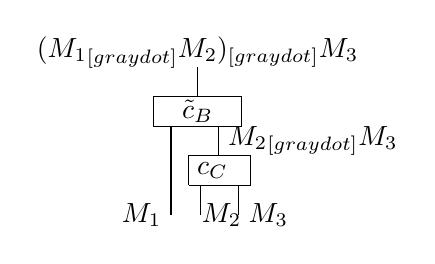
\begin{tikzpicture}[scale=0.75]
\node at (0.75,1.25) {$({M_1}_{\tinydot[gray dot]} {M_2})_{\tinydot[gray dot]} {M_3}$};
\draw (0,0) -- (0,0.5) -- (1.5, 0.5) -- (1.5,0) -- (0,0);
\node at (0.75,0.25) [] {$\tilde{c}_B$};
\draw (0.75,0.5) to  (0.75,1);
\draw (0.3,0) -- (0.3,-1.5)node[left]{$M_1$};
\draw  (1.1,0) to node[right]{${M_2}_{\tinydot[gray dot]}M_3$} (1.1,-0.5);
\draw (0.6,-1) -- (0.6,-0.5) -- (1.65, -0.5) -- (1.65,-1) -- (0.6,-1);
\node at (1,-0.75) [] {$c_C$};
\draw (0.8,-1) to (0.8,-1.5)node[right,xshift=-3pt]{$M_2$}; 
\draw (1.45,-1) -- (1.45,-1.5)node[right]{$M_3$};
\end{tikzpicture}
\end{aligned}
\hspace{.5cm}
\pi_2:=
\begin{aligned}
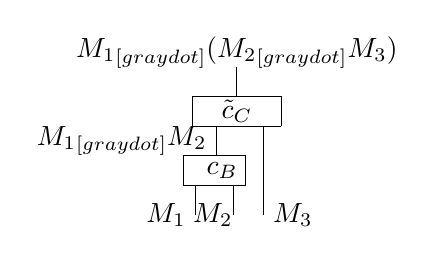
\begin{tikzpicture}[xscale=-0.75, yscale=0.75]
\node at (0.75,1.25) {${M_1}_{\tinydot[gray dot]} ({M_2}_{\tinydot[gray dot]} {M_3})$};
\draw (0,0) -- (0,0.5) -- (1.5, 0.5) -- (1.5,0) -- (0,0);
\node at (0.75,0.25) [] {$\tilde{c}_C$};
\draw (0.75,0.5) -- (0.75,1);
\draw (0.3,0) -- (0.3,-1.5)node [right]{$M_3$};
\draw  (1.1,0) to node[left]{${M_1}_{\tinydot[gray dot]}M_2$} (1.1,-0.5);
\draw (0.6,-1) -- (0.6,-0.5) -- (1.65, -0.5) -- (1.65,-1) -- (0.6,-1);
\node at (1,-0.75) [] {$c_B$};
\draw (0.8,-1) to (0.8,-1.5)node [left,xshift=3pt]{$M_2$}; 
\draw (1.45,-1) to (1.45,-1.5)node[left]{$M_1$};
\end{tikzpicture}
\end{aligned}
\end{equation}

To verify that $\pi_1$ is a coequalised, we first check that it is a cocone of $_{\tinydot [gray dot]}{\bf M_1} \ten {}_{\tinydot[gray dot]}{\bf M_2} \ten \mathid_{M_3}$ and $\mathid_{M_1} \ten {\bf M_2}_{\tinydot[gray dot]} \ten  {\bf M_3}_{\tinydot[gray dot]}$. This follows from the equalities below.

\begin{equation}
\begin{aligned}
\begin{tikzpicture}[xscale=0.8,yscale=0.7]
\node at (0.75,1.25) {$({M_1}_{\tinydot[gray dot]} {M_2})_{\tinydot[gray dot]} {M_3}$};
\draw (0,0) -- (0,0.5) -- (1.5, 0.5) -- (1.5,0) -- (0,0);
\node at (0.75,0.25) [] {$\tilde{c}_B$};
\draw (0.75,0.5) -- (0.75,1);
\draw (0.3,0) to[in=90,out=-90] (-0.1,-1.5);
\draw  (1.1,0) -- (1.1,-0.5);
\draw (0.6,-1) -- (0.6,-0.5) -- (1.65, -0.5) -- (1.65,-1) -- (0.6,-1);
\node at (1.1,-0.75) [] {$c_C$};
\draw (0.8,-1) to (0.8,-1.5); 
\draw (1.45,-1) to[in=90,out=-90] (1.85,-3);
\draw (-0.5,-2) -- (0.3, -2) -- (0.3, -1.5) -- (-0.5,-1.5) -- (-0.5,-2);
\node at (-0.1, -1.75) {$\bf M_1$};
\draw (0.4,-2) -- (1.2,-2) -- (1.2,-1.5) -- (0.4,-1.5) -- (0.4,-2);
\draw (-0.4,-2) to (-0.4,-2.25) node[gray dot]{};
\draw (-0.1,-2) -- (-0.1,-3);
\draw (0.2,-2) -- (0.2,-3);
\draw (0.5,-2) to (0.5,-2.25) node[gray dot]{};
\draw (0.8,-2) to (0.8,-3);
\draw (1.1,-2) to[in=90,out=-90] (1.3,-3);
\node at (0.8,-1.75) {$\bf M_2$};
\node at (-0.1,-3.25) [] {$M_1$};
\node at (0.3,-3.25) [] {$B$};
\node at (0.8,-3.25) [] {$M_2$};
\node at (1.3,-3.25) [] {$C$};
\node at (1.85,-3.25) [] {$M_3$};
\end{tikzpicture}
\end{aligned}
=
\begin{aligned}
\begin{tikzpicture}[xscale=1.2,yscale=0.7]
\node at (0.75,1.25) {$({M_1}_{\tinydot[gray dot]} {M_2})_{\tinydot[gray dot]} {M_3}$};
\draw (0,0) -- (0,0.5) -- (1.5, 0.5) -- (1.5,0) -- (0,0);
\node at (0.75,0.25) [] {$\tilde{c}_B$};
\draw (0.75,0.5) -- (0.75,1);
\draw (0.3,0) to[in=90, out=-90] (0.1,-3.5);
\draw  (1.1,0) -- (1.1,-0.5);
\draw (0.5,-1) -- (0.5,-0.5) -- (1.7, -0.5) -- (1.7,-1) -- (0.5,-1);
\node at (1.1,-0.75) [] {$\bf {M_2}_{\tinydot[gray dot]}M_3$};
\draw (0.6,-1) to[in=90,out=-90] (0.5,-3.5); 
\draw (1.1,-1) -- (1.1,-1.5);
\draw (1.6,-1) to (1.6,-1.25) node[gray dot] {};
\draw (0.7,-2) -- (1.7,-2) -- (1.7,-1.5) -- (0.7,-1.5) -- (0.7,-2);
\node at (1.1,-1.75) {$c_C$};
\draw (0.9,-2) -- (0.9,-3.5);
\draw (1.5,-2) -- (1.5,-2.5);
\draw (1.1,-3) -- (1.9,-3) -- (1.9,-2.5) -- (1.1,-2.5) -- (1.1,-3);
\node at (1.5,-2.75) {$\bf M_3$};
\draw (1.2,-3) -- (1.2,-3.5);
\draw (1.5,-3) -- (1.5,-3.5);
\draw (1.8,-3) to (1.8,-3.25) node[gray dot]{};
\node at (0.1,-3.75) [] {$M_1$};
\node at (0.5,-3.75) [] {$B$};
\node at (0.9,-3.75) [] {$M_2$};
\node at (1.2,-3.75) [] {$C$};
\node at (1.5,-3.75) [] {$M_3$};
\end{tikzpicture}
\end{aligned}
=
\begin{aligned}
\begin{tikzpicture}[xscale=1.2,yscale=0.7]
\node at (0.75,1.25) {$({M_1}_{\tinydot[gray dot]} {M_2})_{\tinydot[gray dot]} {M_3}$};
\draw (0,0) -- (0,0.5) -- (1.5, 0.5) -- (1.5,0) -- (0,0);
\node at (0.75,0.25) [] {$\tilde{c}_B$};
\draw (0.75,0.5) -- (0.75,1);
\draw (0.2,0) to[in=90, out=-90] (-0.2,-3.5);
\draw  (1.1,0) -- (1.1,-0.5);
\draw (0.5,-1) -- (0.5,-0.5) -- (1.7, -0.5) -- (1.7,-1) -- (0.5,-1);
\node at (1.1,-0.75) [] {$c_C$};
\draw (0.6,-1) -- (0.6,-1.5); 
\draw (1.6,-1) -- (1.6,-1.5);
\draw (0.2,-2) -- (1,-2) -- (1,-1.5) -- (0.2,-1.5) -- (0.2,-2);
\node at (0.6,-1.75) {$\bf M_2$};
\draw (0.3,-2) to [in=90,out=-90] (0.2,-3.5);
\draw (0.6,-2) -- (0.6,-3.5);
\draw (0.9,-2) to (0.9,-2.25) node[gray dot] {};
\draw (1.2,-2) -- (2,-2) -- (2,-1.5) -- (1.2,-1.5) -- (1.2,-2);
\node at (1.6,-1.75) {$\bf M_3$};
\draw (1.3,-2) to (1.3,-2.25) node[gray dot] {};
\draw (1.6,-2) -- (1.6,-2.5);
\draw (1.9,-2) to (1.9,-2.25) node[gray dot] {};
\draw (1.1,-3) -- (1.9,-3) -- (1.9,-2.5) -- (1.1,-2.5) -- (1.1,-3);
\node at (1.5,-2.75) {$\bf M_3$};
\draw (1.2,-3) to[in=90,out=-90] (1.1,-3.5);
\draw (1.5,-3) -- (1.5,-3.5);
\draw (1.8,-3) to (1.8,-3.25) node[gray dot]{};
\node at (-0.2,-3.75) [] {$M_1$};
\node at (0.2,-3.75) [] {$B$};
\node at (0.6,-3.75) [] {$M_2$};
\node at (1.1,-3.75) [] {$C$};
\node at (1.5,-3.75) [] {$M_3$};
\end{tikzpicture}
\end{aligned}
=
\begin{aligned}
\begin{tikzpicture}[xscale=1.2,yscale=0.7]
\node at (0.75,1.25) {$({M_1}_{\tinydot[gray dot]} {M_2})_{\tinydot[gray dot]} {M_3}$};
\draw (0,0) -- (0,0.5) -- (1.5, 0.5) -- (1.5,0) -- (0,0);
\node at (0.75,0.25) [] {$\tilde{c}_B$};
\draw (0.75,0.5) -- (0.75,1);
\draw (0.2,0) to[in=90, out=-90] (-0.2,-3);
\draw  (1.1,0) -- (1.1,-0.5);
\draw (0.5,-1) -- (0.5,-0.5) -- (1.7, -0.5) -- (1.7,-1) -- (0.5,-1);
\node at (1.1,-0.75) [] {$c_C$};
\draw (0.6,-1) -- (0.6,-1.5); 
\draw (1.6,-1) -- (1.6,-1.5);
\draw (0.2,-2) -- (1,-2) -- (1,-1.5) -- (0.2,-1.5) -- (0.2,-2);
\node at (0.6,-1.75) {$\bf M_2$};
\draw (0.3,-2) to [in=90,out=-90] (0.2,-3);
\draw (0.6,-2) -- (0.6,-3);
\draw (0.9,-2) to (0.9,-2.25) node[gray dot] {};
\draw (1.2,-2) -- (2,-2) -- (2,-1.5) -- (1.2,-1.5) -- (1.2,-2);
\node at (1.6,-1.75) {$\bf M_3$};
\draw (1.3,-2) to [in=90, out=-90] (1.2,-3) {};
\draw (1.6,-2) -- (1.6,-3);
\draw (1.9,-2) to (1.9,-2.25) node[gray dot] {};
\node at (-0.2,-3.25) [] {$M_1$};
\node at (0.2,-3.25) [] {$B$};
\node at (0.6,-3.25) [] {$M_2$};
\node at (1.2,-3.25) [] {$C$};
\node at (1.6,-3.25) [] {$M_3$};
\end{tikzpicture}
\end{aligned}
\end{equation}

The last step for showing that $\pi_1$ is a coequaliser, is to prove that if we have another cocone $f$, then $f$ factorises through $\pi_1$. Let $f$ be such a cocone. First of all, it is easy to show that the two equalities below hold, expressing that $f$ is a cocone of the respective pairs of morphisms. One obtains this by plugging  the unit on $B$ or $C$, respectively, in the cocone equality for $f$ and then applying the unit laws for modules.

\begin{equation}
\begin{aligned}
\begin{tikzpicture}[xscale=0.8,yscale=0.7]
\node at (0.75,1.25) {$({M_1}_{\tinydot[gray dot]} {M_2})_{\tinydot[gray dot]} {M_3}$};
\draw (0,0) -- (0,0.5) -- (1.5, 0.5) -- (1.5,0) -- (0,0);
\node at (0.75,0.25) [] {$f$};
\draw (0.75,0.5) -- (0.75,1);
\draw (0.3,0) to[in=90,out=-90] (-0.1,-3);
\draw (0.8,0) to (0.8,-1.5); 
\draw (1.35,0) to[in=90,out=-90] (1.85,-3);
\draw (0.4,-2) -- (1.2,-2) -- (1.2,-1.5) -- (0.4,-1.5) -- (0.4,-2);
\draw (0.5,-2) to (0.5,-2.25) node[gray dot]{};
\draw (0.8,-2) to (0.8,-3);
\draw (1.1,-2) to[in=90,out=-90] (1.3,-3);
\node at (0.8,-1.75) {$\bf M_2$};
\node at (-0.1,-3.25) [] {$M_1$};
\node at (0.8,-3.25) [] {$M_2$};
\node at (1.3,-3.25) [] {$C$};
\node at (1.85,-3.25) [] {$M_3$};
\end{tikzpicture}
\end{aligned}
=
\begin{aligned}
\begin{tikzpicture}[xscale=0.8, yscale=0.7]
\node at (0.75,1.25) {$({M_1}_{\tinydot[gray dot]}{M_2})_{\tinydot[gray dot]} {M_3}$};
\draw (0,0) -- (0,0.5) -- (1.5, 0.5) -- (1.5,0) -- (0,0);
\node at (0.75,0.25) [] {$f$};
\draw (0.75,0.5) -- (0.75,1);
\draw (0.2,0) to[in=90, out=-90] (-0.2,-3);
\draw (0.6,0) -- (0.6,-3); 
\draw (1.35,0) to [in=90,out=-90] (1.6,-1.5);
\draw (0.6,-2) -- (0.6,-3);
\draw (1.2,-2) -- (2,-2) -- (2,-1.5) -- (1.2,-1.5) -- (1.2,-2);
\node at (1.6,-1.75) {$\bf M_3$};
\draw (1.3,-2) to [in=90, out=-90] (1.2,-3) {};
\draw (1.6,-2) -- (1.6,-3);
\draw (1.9,-2) to (1.9,-2.25) node[gray dot] {};
\node at (-0.2,-3.25) [] {$M_1$};
\node at (0.6,-3.25) [] {$M_2$};
\node at (1.2,-3.25) [] {$C$};
\node at (1.6,-3.25) [] {$M_3$};
\end{tikzpicture}
\end{aligned}
\hspace{1cm}
\begin{aligned}
\begin{tikzpicture}[xscale=0.8,yscale=0.7]
\node at (0.75,1.25) {$({M_1}_{\tinydot[gray dot]} {M_2})_{\tinydot[gray dot]} {M_3}$};
\draw (0,0) -- (0,0.5) -- (1.5, 0.5) -- (1.5,0) -- (0,0);
\node at (0.75,0.25) [] {$f$};
\draw (0.75,0.5) -- (0.75,1);
\draw (0.3,0) to[in=90,out=-90] (-0.1,-1.5);
\draw (0.8,0) to (0.8,-3); 
\draw (1.35,0) to[in=90,out=-90] (1.85,-3);
\draw (-0.5,-2) -- (0.3, -2) -- (0.3, -1.5) -- (-0.5,-1.5) -- (-0.5,-2);
\node at (-0.1, -1.75) {$\bf M_1$};
\draw (-0.4,-2) to (-0.4,-2.25) node[gray dot]{};
\draw (-0.1,-2) -- (-0.1,-3);
\draw (0.2,-2) -- (0.2,-3);
\node at (-0.1,-3.25) [] {$M_1$};
\node at (0.3,-3.25) [] {$B$};
\node at (0.8,-3.25) [] {$M_2$};
\node at (1.85,-3.25) [] {$M_3$};
\end{tikzpicture}
\end{aligned}
=
\begin{aligned}
\begin{tikzpicture}[xscale=0.8,yscale=0.7]
\node at (0.75,1.25) {$({M_1}_{\tinydot[gray dot]} {M_2})_{\tinydot[gray dot]} {M_3}$};
\draw (0,0) -- (0,0.5) -- (1.5, 0.5) -- (1.5,0) -- (0,0);
\node at (0.75,0.25) [] {$f$};
\draw (0.75,0.5) -- (0.75,1);
\draw (0.2,0) to[in=90, out=-90] (-0.2,-3);
\draw (0.6,0) -- (0.6,-1.5); 
\draw (1.35,0) to [in=90,out=-90] (1.6,-3);
\draw (0.2,-2) -- (1,-2) -- (1,-1.5) -- (0.2,-1.5) -- (0.2,-2);
\node at (0.6,-1.75) {$\bf M_2$};
\draw (0.3,-2) to [in=90,out=-90] (0.2,-3);
\draw (0.6,-2) -- (0.6,-3);
\draw (0.9,-2) to (0.9,-2.25) node[gray dot] {};
\node at (-0.2,-3.25) [] {$M_1$};
\node at (0.2,-3.25) [] {$B$};
\node at (0.6,-3.25) [] {$M_2$};
\node at (1.6,-3.25) [] {$M_3$};
\end{tikzpicture}
\end{aligned}
\end{equation}



It follows from the first equality that $f$ factorises through $\id_{M_1} \ten c_{C}$. This means that there exists a morphism $f'$ such that $f = f' \verc (\id_{M_1} \ten c_{C})$. 
From the second statement we deduce that $f'$ factorises through $\tilde{c}_B$, which finishes our proof. The equations below and the fact that $\mathid \ten c_C$ is epic imply that $f'$ is a cocone of $_{\tinydot[gray dot]}{\bf M_1} \otimes \id_{M_2} \otimes \id_{M_3}$ and $\id_{M_1} \otimes {\bf M_{2\tinydot[gray dot]}M_3}_{\tinydot[gray dot]}$. 
As a result, $f'$ factorises through  $\id_{M_1} \ten \tilde{c}_B$. Hence, there exists a morphism $f''$ such that $f = f'' \verc \tilde{c}_B \verc  (\id_{M_1} \ten c_C) = f'' \verc \pi_1$. One can use a similar argument to show that $\pi_2$ is a coequaliser.  
 
 
\begin{equation}
\begin{aligned}
\begin{tikzpicture}[yscale=0.78, xscale=0.7]
\draw (2,2.5) -- (2,3);
\draw (0.8,2) -- (3.2,2) -- (3.2,2.5) -- (0.8,2.5) -- (0.8,2);
\node at (2,2.25) {$f'$};
\draw (1,2) -- (1,1.5);
\draw (2.5,2) -- (2.5,0.5);
\draw (0.6,1) -- (1.4,1) -- (1.4,1.5) -- (0.6,1.5) -- (0.6,1);
\node at (1,1.25) {$\bf M_1$};
\draw (1.8,0) -- (3.2,0) -- (3.2,0.5) -- (1.8,0.5) -- (1.8,0);
\node at (2.5,0.25) {$c_C$};
\draw (0.7,1) to (0.7,0.75) node[gray dot] {};
\draw (1,1) to (1,-0.5);
\draw (1.3,1) to [in=90,out=-90] (1.5,-0.5);
\node at (1,-0.75) {$M_1$};
\node at (1.5,-0.75) {$B$};
\draw (2,0) -- (2,-0.5);
\draw (3,0) -- (3,-0.5);
\node at (2,-0.75) {$M_2$};
\node at (3,-0.75) {$M_3$};
\end{tikzpicture}
\end{aligned}
=
\begin{aligned}
\begin{tikzpicture}[yscale=0.78, xscale=0.7]
\draw (2,2.5) -- (2,3);
\draw (0.8,2) -- (3.2,2) -- (3.2,2.5) -- (0.8,2.5) -- (0.8,2);
\node at (2,2.25) {$f$};
\draw (1,2) -- (1,1.5);
\draw (2,2) -- (2,-0.5);
\draw (3,2) -- (3,-0.5);
\draw (0.6,1) -- (1.4,1) -- (1.4,1.5) -- (0.6,1.5) -- (0.6,1);
\node at (1,1.25) {$\bf M_1$};
\draw (0.7,1) to (0.7,0.75) node[gray dot] {};
\draw (1,1) to (1,-0.5);
\draw (1.3,1) to [in=90,out=-90](1.5,-0.5);
\node at (1,-0.75) {$M_1$};
\node at (1.5,-0.75) {$B$};
\node at (2,-0.75) {$M_2$};
\node at (3,-0.75) {$M_3$};
\end{tikzpicture}
\end{aligned}
=
\begin{aligned}
\begin{tikzpicture}[yscale=0.78, xscale=0.7]
\draw (2,2.5) -- (2,3);
\draw (0.8,2) -- (3.2,2) -- (3.2,2.5) -- (0.8,2.5) -- (0.8,2);
\node at (2,2.25) {$f$};
\draw (1,2) -- (1,-0.5);
\draw (2,2) -- (2,1.5);
\draw (3,2) -- (3,1.5);
\draw (1.6,1) -- (2.4,1) -- (2.4,1.5) -- (1.6,1.5) -- (1.6,1);
\node at (2,1.25) {$\bf M_2$};
\draw (2.6,1) -- (3.4,1) -- (3.4,1.5) -- (2.6,1.5) -- (2.6,1);
\node at (3,1.25) {$\bf M_3$};
\draw (1.7,1) to [in=90,out=-90](1.5,-0.5);
\draw (2,1) -- (2,-0.5);
\draw (2.3,1) to (2.3,0.75) node[gray dot] {};
\node at (1,-0.75) {$M_1$};
\draw (2.7,1) to (2.7,0.75)node[gray dot]{};
\draw (3,1) -- (3,-0.5);
\draw (3.3,1) to (3.3,0.75) node[gray dot] {};
\node at (1.5,-0.75) {$B$};
\node at (2,-0.75) {$M_2$};
\node at (3,-0.75) {$M_3$};
\end{tikzpicture}
\end{aligned}
=
\begin{aligned}
\begin{tikzpicture}[yscale=0.78, xscale=0.7]
\draw (2,2.5) -- (2,3);
\draw (0.8,2) -- (3.2,2) -- (3.2,2.5) -- (0.8,2.5) -- (0.8,2);
\node at (2,2.25) {$f'$};
\draw (1,2) -- (1,-0.5);
\draw (2.5,2) -- (2.5,1.5);
\draw (1.8,1.5) -- (3.2,1.5) -- (3.2,1) -- (1.8,1) -- (1.8,1.5);
\node at (2.5,1.25){$c_C$};
\draw (2,1) -- (2,0.5);
\draw (3,1) -- (3,0.5);
\draw (1.6,0) -- (2.4,0) -- (2.4,0.5) -- (1.6,0.5) -- (1.6,0);
\node at (2,0.25) {$\bf M_2$};
\draw (2.6,0) -- (3.4,0) -- (3.4,0.5) -- (2.6,0.5) -- (2.6,0);
\node at (3,0.25) {$\bf M_3$};
\draw (1.7,0) to [in=90,out=-90] (1.5,-0.5);
\draw (2,0) -- (2,-0.5);
\draw (2.3,0) to (2.3,-0.25) node[gray dot] {};
\node at (1,-0.75) {$M_1$};
\draw (2.7,0) to (2.7,-0.25)node[gray dot]{};
\draw (3,1) -- (3,-0.5);
\draw (3.3,0) to (3.3,-0.25) node[gray dot] {};
\draw (2,0) -- (2,-0.5);
\draw (3,0) -- (3,-0.5);
\node at (1.5,-0.75) {$B$};
\node at (2,-0.75) {$M_2$};
\node at (3,-0.75) {$M_3$};
\end{tikzpicture}
\end{aligned}
=
\begin{aligned}
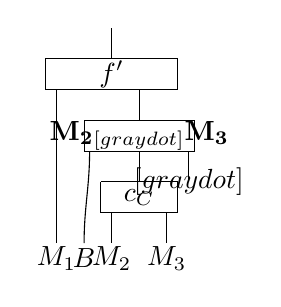
\begin{tikzpicture}[yscale=0.78, xscale=0.7]
\draw (2,2.5) -- (2,3);
\draw (0.8,2) -- (3.2,2) -- (3.2,2.5) -- (0.8,2.5) -- (0.8,2);
\node at (2,2.25) {$f'$};
\draw (1,2) -- (1,-0.5);
\draw (2.5,2) -- (2.5,1.5);
\draw (1.5,1.5) -- (3.5,1.5) -- (3.5,1) -- (1.5,1) -- (1.5,1.5);
\node at (2.5,1.25) {${\bf M_2}_{\tinydot[gray dot]}{\bf M_3}$};
\draw (2.5,1) -- (2.5,0.5);
\draw (1.6,1) to [in=90,out=-90] (1.5,-0.5);
\draw (3.4,1) to (3.4,0.5); 
\node at (3.4,0.5) {$\tinydot[gray dot]$};
\draw (2,0) to (2,-0.5);
\draw (3,0) to (3,-0.5);
\draw (1.8, 0.5) -- (3.2,0.5) -- (3.2,0) -- (1.8,0) -- (1.8,0.5);
\node at (2.5,0.25) {$c_C$};
\node at (1.5,-0.75) {$B$};
\node at (1,-0.75) {$M_1$};
\node at (2,-0.75) {$M_2$};
\node at (3,-0.75) {$M_3$};
\end{tikzpicture}
\end{aligned}
\end{equation}



The components of the {\bf left unitor} $l_{\bf M}: U_A \odot {\bf M} \rightarrow {\bf M}$ are given by $(\mathid, l_{M}, \mathid)$, where $ l_{M}$ is defined as follows: By the module laws, ${\bf M}_{\tinydot[gray dot]}: A \ten M \rightarrow M$ is a coequaliser of the maps $_{\tinydot[gray dot]}{\bf A} \ten \mathid_{M}$ and $\mathid_{A} \ {\bf M}_{\tinydot[gray dot]}$. The canonical isomorphisms between ${\bf M}$ and ${\bf A}_{\tinydot[gray dot]}{\bf M}$ is the middle component of $l_{\bf M}$, and naturality of $l$ follows from commutativity of the diagram below. We can define $r$, and prove its naturality, in a similar way.
    
\begin{tikzpicture}[xscale=4,yscale=2]
 \node (tl) at (0,1) {$A \ten A \ten M$};
 \node (bl) at (0,0) {$B \ten B \ten N$};
  \node (tm) at (1,1) {$A \ten M$};
 \node (bm) at (1,0) {$B \ten N$};
\draw[->] ([yshift=1.5pt] tl.east) to node[above] {${}_{\tinydot[gray dot]}U_{A} \ten \mathid_M$} ([yshift=1.5pt] tm.west);
\draw[->] ([yshift=-1.5pt] tl.east) to node[below] {$\mathid_{A} \ten {\bf M}_{\tinydot[gray dot]}$} ([yshift=-1.5pt] tm.west);
\draw[->] ([yshift=1.5pt] bl.east) to node[above] {$_{\tinydot[gray dot]}U_A \ten \mathid_N$} ([yshift=1.5pt] bm.west);
\draw[->] ([yshift=-1.5pt] bl.east) to node[below] {$\mathid_{B} \ten {N}_{\tinydot[gray dot]}$} ([yshift=-1.5pt] bm.west);
 \node (r1) at (2,1.25) {$A_{\tinydot[gray dot]} M$};
 \node (r2) at (1.6,0.75) {$M$};
  \node (r3) at (2,0.25) {$B_{\tinydot[gray dot]} N$};
 \node (r4) at (1.6,-0.25) {$N$};
 \draw[->] (tm) to node[above] {$c_M$} (r1.west);
 \draw[->] (tm) to node[below] {${\bf M}_{\tinydot[gray dot]}$} (r2);
  \draw[->] (bm) to node[above] {$c_N$} (r3.west);
 \draw[->] (bm) to node[below] {${\bf N}_{\tinydot[gray dot]}$} (r4);
  \draw[->, dashed] (r1) to node[left] {$l_M$} (r2);
 \draw[->, dashed] (r3) to node[right] {$l_N$} (r4);
  \draw[->, dashed] (r1) to node[right] {$f \tinydot[gray dot] g$} (r3);
 \draw[->, dashed, cross] (r2) to node[left, yshift=10pt] {$g$} (r4);
 \draw[->] (tl) to node[left] {$f \ten f \ten g$} (bl);
 \draw[->] (tm) to node[left] {$f \ten g$} (bm);
\end{tikzpicture}
\end{proof}


\subsection{The braided monoidal structure of $\bAlg$}\label{sec:brmonDalg}

In this section we will prove that $\bAlg({\bf C})$ is a braided monoidal double category and that it is symmetric whenever ${\bf C}$ is symmetric.

\begin{prop}\label{lem:algsymmon}
Let ${\bf C}$ be a braided or symmetric monoidal category, the double category $\bAlg({\cat C})$ of algebras, bimodules and bimodule homomorphisms in {\bf C} is braided or symmetric monoidal, respectively.
\end{prop}

\begin{proof}

We have seen that $\D_0$ and $\D_1$ are braided or symmetric monoidal when ${\bf C}$ is braided or symmetric. Clearly, $S$ and $T$ are strict monoidal functors preserving the associativity and unit constraints, and $U_I$ is the monoidal unit of $D_1$, when $I$ is the monoidal unit of $D_0$.

Unfolding definitions shows that the globular isomorphism $\fu$ from $U \circ \tens$ to $\tens \circ (U \times U)$ is the identity. We define the exchange law, ${\bf \fx}$, between the functors $\odot$ and $\tens$ as $(\mathid, \xi, \mathid)$, where $\xi$ is the unique morphism completing the commuting diagram below.
In this diagram, $c$, $c_M$, and $c_N$ are the coequalisers defining  $({M_1} \ten {N_1})_{\tinydot[gray dot]}({M_2} \ten {N_2})$, ${M_1}_{\tinydot[gray dot]} M_2$, and ${N_1}_{\tinydot[gray dot]} N_2$, respectively. By a similar argument given while defining the associator ${\bf a}$ for the double category, one can show that $c_M \ten c_N$ is the coequaliser of the lower two parallel maps in the diagram. The two leftmost vertical morphisms are natural isomorphisms constructed from swam maps. For later use, we will denote the middle morphism by $\hat{\sigma}$.

\begin{equation}\label{def:xi}
  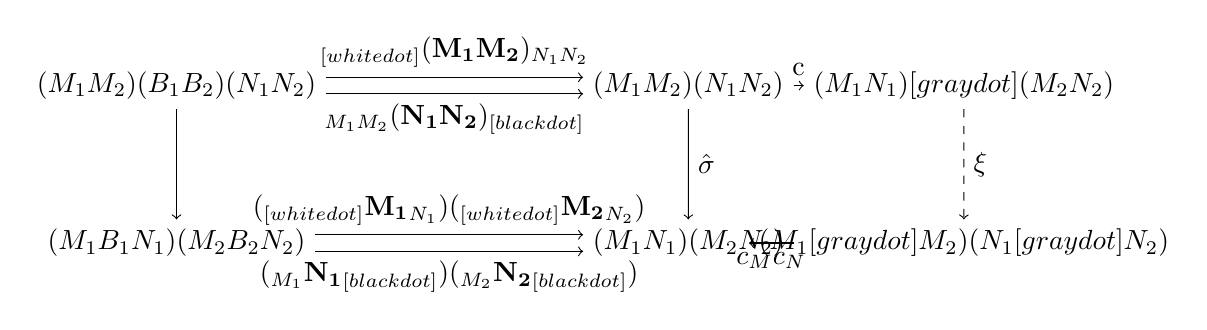
\begin{tikzpicture}[xscale=5, yscale=2, thin]
    \node (tl) at (-.3,1) {$(M_1 \tens M_2) \ten (B_1 \tens B_2) \ten (N_1 \tens N_2)$};
    \node (bl) at (-.3,0) {$(M_1 \ten B_1 \ten N_1) \tens (M_2 \ten B_2 \ten N_2)$};
    \node (t) at (1,1) {$(M_1 \tens M_2) \ten (N_1 \tens N_2)$};
    \node (b) at (1,0) {$(M_1 \ten N_1) \tens (M_2 \ten N_2)$};
    \node (tr) at (1.7,1) {$({M_1} \tens {N_1}) \tinydot[gray dot] ({M_2} \tens {N_2})$};
    \node (br) at (1.7,0) {$({M_1} \tinydot[gray dot] {M_2}) \tens ({N_1} \tinydot[gray dot] {N_2})$};
    \draw[->] (tl) to node[left] {$\iso$} (bl);
    \draw[->] (t) to node[right] {$\iso \hat{\sigma} $} (b);
    \draw[->, dashed] (tr) to node[right] {$\iso {\xi} $} (br);
    \draw[->] (t) to node[above] {c} (tr);
    \draw[->] (b) to node[below] {$c_M \tens c_N$} (br);
    \draw[->] ([yshift=1.5pt]tl.east) to node[above] {${}_{\tinydot[white dot]}(\mathbf{M_1} \tens \mathbf{M_2}) \ten \mathid_{N_1 \tens N_2}$} ([yshift=1.5pt]t.west);
    \draw[->] ([yshift=-1.5pt]tl.east) to node[below] {$\mathid_{M_1 \tens M_2} \ten (\mathbf{N_1} \tens \mathbf{N_2})_{\tinydot[black dot]}$} ([yshift=-1.5pt]t.west);
    \draw[->] ([yshift=1.5pt]bl.east) to node[above] {$
    ({}_{\tinydot[white dot]}\mathbf{M_1} \ten \mathid_{N_1}) \tens ({}_{\tinydot[white dot]}\mathbf{M_2} \ten \mathid_{N_2})$} ([yshift=1.5pt]b.west);
    \draw[->] ([yshift=-1.5pt]bl.east) to node[below] {$(\mathid_{M_1} \ten \mathbf{N_1}_{\tinydot[black dot]}) \tens (\mathid_{M_2} \ten \mathbf{N_2}_{\tinydot[black dot]})$} ([yshift=-1.5pt]b.west);
  \end{tikzpicture}
 \end{equation}


It is left to prove is that the diagrams given in points (iv),(v),(vi), and (ix) of Definition ~\ref{def:symmondoub} commute. Because $\fu$ and $\fx$ are globular, it suffices to verify commutativity of the diagrams for the middle component of the extended module homomorphisms.

The first equation of (iv) corresponds to the front square of the diagram below. The unlabelled arrows represent the coequalisers defining their target object. The back square commutes by coherence of the braided monoidal category {\cat C}. The squares on the sides commute by definition of  $\xi$, ${\bf a}$ and $\tinydot[gray dot]$. It follows that the front square must commute as well, which is what we wanted to prove.
\begin{equation}
\begin{tikzpicture}[xscale=3.2, yscale=2]
%lowersquare
\node (b1) at (0,0) [] {$(M_1 \tens N_1) \hor ((M_2 \hor M_3) \tens (N_2 \hor N_3))$};
\node (b2) at (2,0) [] {$(M_1 \hor (M_2 \hor M_3) \tens (N_1 \hor (N_2 \hor N_3))$};
\node (b3) at (1,-0.5) [] {$(M_1 \tens {N_1})_{\tinydot[gray dot]} (({M_2}_{\tinydot[gray dot]} M_3) \tens ({N_2}_{\tinydot[gray dot]} N_3))$};
\node (b4) at (3,-0.5) [] {$({M_1}_{\tinydot[gray dot]} ({M_2}_{\tinydot[gray dot]} M_3 )) \tens ({N_1}_{\tinydot[gray dot]} ({N_2}_{\tinydot[gray dot]} N_3))$}; 
\draw[->] (b1) to node[above, xshift=7pt] {$\hat{\sigma}$} (b2);
\draw[->] (b3) to node[above] {$\xi$} (b4);
\draw[->] (b1) to node[above] {} (b3); 
\draw[->] (b2) to node[above] {} (b4);
%middlesquare
\node (m1) at (0,1.5) [] {$(M_1 \tens N_1) \hor ((M_2 \tens N_2)) \hor (M_3 \tens N_3))$};
\node (m2) at (2,1.5) [] {$((M_1 \hor M_2) \hor M_3) \tens ((N_1 \hor N_2) \hor N_3)$};
\node (m3) at (1,1) [] {$(M_1 \tens {N_1})_{\tinydot[gray dot]} ((M_2 \tens {N_2})_{\tinydot[gray dot]} (M_3 \tens N_3))$};
\node (m4) at (3,1) [] {$({M_1}_{\tinydot[gray dot]} {M_2})_{\tinydot[gray dot]} {M_3}) \tens (({N_1}_{\tinydot[gray dot]}N_2)_{\tinydot[gray dot]} N_3)$};
\draw[->] (m1) to node[above] {} (m3); 
\draw[->] (m2) to node[above] {} (m4);
%lowervertical
\draw[->] (m1) to node[left] {$\mathid \hor \hat{\sigma}$} (b1); 
\draw[->] (m2) to node[left] {$\alpha \tens \alpha$} (b2);
\draw[->, cross] (m3) to node[left, yshift=8pt] {$\mathid \tinydot[gray dot] \xi$} (b3); 
\draw[->] (m4) to node[left] {$a \tens a$} (b4);
%uppersquare
\node (u1) at (0,3) [] {$((M_1 \tens N_1) \hor (M_2 \tens N_2)) \hor (M_3 \tens N_3)$};
\node (u2) at (2,3) [] {$((M_1 \hor M_2) \tens (N_1 \hor N_2)) \hor (M_3 \tens N_3)$};
\node (u3) at (1,2.5) [] {$((M_1 \tens N_1)_{\tinydot[gray dot]}(M_2 \tens N_2))_{\tinydot[gray dot]}(M_3 \tens N_3)$};
\node (u4) at (3,2.5) [] {$(({M_1}_{\tinydot[gray dot]} M_2) \tens ({N_1}_{\tinydot[gray dot]} N_2))_{\tinydot[gray dot]} (M_3 \tens N_3)$};
\draw[->] (u1) to node[left] {$\alpha$} (m1); 
\draw[->] (u2) to node[left] {$\hat{\sigma}$} (m2);
\draw[->, cross] (u3) to node[left] {$a$} (m3); 
\draw[->] (u4) to node[left] {$\xi$} (m4);
\draw[->, cross] (u3) to node[above, xshift=8pt] {$\xi_{\tinydot[gray dot]} \mathid$} (u4); 
\draw[->] (u1) to node[above] {$\hat{\sigma} \hor \mathid$} (u2);
\draw[->] (u1) to node[below] {} (u3); 
\draw[->, cross] (u2) to node[above] {} (u4);
\end{tikzpicture}
\end{equation}

All other equations concerning $\xi$ are proven in the same way. These are the second and third equation of (iv), the first equation of (v), the first and the third equation of (vi), and the first equation of (ix).
It is easy to see that the other equations, which concern $\fu$ hold, keeping in mind that $\fu$ is the identity, and $U_{\alpha_{A,B,C}} = \alpha_{U_A,U_B,U_C}$, $U(\rho_A) = \rho_{U_A}$, $U(\lambda_A) = \lambda_{U_A}$, and $\sigma_{U_A,U_B} = U(\sigma_{A,B})$.
\end{proof}

\subsection{Companions and conjoints in $\bAlg$}\label{sec:fibDalg}
Finally, we will prove that $\bAlg(\cat C$) is fibrant.  This is the last step we need to take to show that we can lift $\bAlg({\cat C})$ to obtain the bicategory ${\cA}lg({\cat C})$, which preserves any braided monoidal structure.

\begin{lem}\label{lem:algfib}
Let ${\bf C}$ be a braided monoidal category. The double category $\bAlg({\cat C})$ is fibrant.
\end{lem}

\begin{proof}
Let $f$ be a morphism of ${\lD_0}$. The companion of $f$ is defined by the following data: 

\begin{equation}\label{eq:companion}
\hat{\bf f}:= 
\begin{aligned}
 \begin{tikzpicture}[scale=0.6] 
\draw (0.5,-0.5)node[below]{$A$} -- (0.5, -0.2);
\draw (0.2,-0.2) -- (0.8,-0.2) -- (0.8,0.7) -- (0.2,0.7) -- (0.2,-0.2);
\draw (0.5,0.7) to[out=90,in=160] (1.2,1.2) node[gray dot] {};
\draw (1.2,-0.5) node[below]{$B$} to (1.2,1.2);
\draw (1.9,0.7) to[out=90, in=20] (1.2,1.2){};
\draw (1.9,0.7)  to (1.9,-0.5)node [below]{$B$};
\draw (1.2,1.9) -- (1.2,1.2){};
\node at (0.5,0.25)[] {$f$};
\node at (1.2,2.1)[]{$B$};
\end{tikzpicture}
\end{aligned}
\quad \quad {\bf \eta_{\hat{f}}} := (id_A, f, f)
\quad \quad {\bf \epsilon_{\hat{f}}} := (f, \mathid_B, \mathid_B)
\end{equation}

The first equation of ~\ref{eq:compeqn} holds because ${\bf \epsilon_{\hat{f}} \circ \eta_{\hat{f}}} = (f,f,f) = {\bf U}_f$. The left-hand-side of the second equation corresponds to ${\bf \eta_{\hat{f}} \odot \epsilon_{\hat{f}}}= (id_A, f\tinydot[gray dot] \mathid_B, \mathid_B): {{\bf U}_A}_{\tinydot[gray dot]} \hat{\bf f} \rightarrow \hat{\bf f}_{\tinydot[gray dot]}{\bf U}_B$, where $f \tinydot[gray dot] \mathid_B$: is the unique map that makes back of the diagram below commute.  

\begin{tikzpicture}[xscale=4,yscale=2]
 \node (tl) at (0,1) {$A \ten A \ten B$};
 \node (bl) at (0,0) {$B \ten B \ten B$};
  \node (tm) at (1,1) {$A \ten B$};
 \node (bm) at (1,0) {$B \ten B$};
\draw[->] ([yshift=1.5pt] tl.east) to node[above] {${}_{\tinydot[white dot]}U_A \ten \mathid_B$} ([yshift=1.5pt] tm.west);
\draw[->] ([yshift=-1.5pt] tl.east) to node[below] {$\mathid_{A} \ten \hat{f}_{\tinydot[gray dot]}$} ([yshift=-1.5pt] tm.west);
\draw[->] ([yshift=1.5pt] bl.east) to node[above] {$_{\tinydot[white dot]}\hat{f} \ten \mathid_B$} ([yshift=1.5pt] bm.west);
\draw[->] ([yshift=-1.5pt] bl.east) to node[below] {$\mathid_{B} \ten {U_B}_{\tinydot[gray dot]}$} ([yshift=-1.5pt] bm.west);
 \node (r1) at (2,1.25) {$A_{\tinydot[gray dot]} B$};
 \node (r2) at (1.6,0.75) {$B$};
  \node (r3) at (2,0.25) {$B_{\tinydot[gray dot]} B$};
 \node (r4) at (1.6,-0.25) {$B$};
 \draw[->] (tm) to node[above] {$c_A$} (r1.west);
 \draw[->] (tm) to node[below] {$\hat{f}_{\tinydot[gray dot]}$} (r2);
  \draw[->] (bm) to node[above,xshift=-4pt] {$c_B$} (r3.west);
 \draw[->] (bm) to node[below] {$_{\tinydot[white dot]}\hat{f}$} (r4);
  \draw[->, dashed] (r1) to node[left] {$l_{\hat{f}}$} (r2);
 \draw[->, dashed] (r3) to node[right] {$r_{\hat{f}}$} (r4);
  \draw[->, dashed] (r1) to node[right] {$f \tinydot[gray dot] \mathid_B$} (r3);
 \draw[->, dashed, cross] (r2) to node[right,yshift=7pt] {$\mathid_B$} (r4);
 \draw[->] (tl) to node[left] {$f \ten f \ten \mathid_B$} (bl);
 \draw[->] (tm) to node[left] {$f \ten \mathid_B$} (bm);
\end{tikzpicture}

We need to show that $f\tinydot[gray dot] \id_B \iso  \mathid_B$. In this diagram, $c_A$ and $c_B$ are the coequalisers defining ${{\bf U}_A}_{\tinydot[gray dot]} \hat{\bf f}$ and $\hat{\bf f}_{\tinydot[gray dot]}{\bf U}_B$, respectively.
It is easy to check that $\hat{f}_{\tinydot[gray dot]}$ and $_{\tinydot[white dot]}{\hat{f}}$ are coequalisers as well. The morphisms $\id_B$, $l_{\hat{f}}$ and $r_{\hat{f}}$ are the unique morphisms that make all diagrams commute. It follows from coherence of double categories that $f \tinydot[gray dot] \mathid_B \iso \mathid_B$, and thus $\eta_{\hat{f}} \odot \epsilon_{\hat{f}} \iso 1_{\hat{f}}$.

This simultaneously proves that $f$ has a conjoint, because $\bAlg({\bf C}^{h* op}) \cong$ $\bAlg({\cat C})$.
\end{proof}

\begin{eg}
When we take the category $\mathcal{A}B$ of Abelian groups and group homomorphisms as our symmetric monoidal category, we obtain the double category $\cMod$ of rings, ring homomorphisms, bimodules and bimodule homomorphisms. As a consequence of Lemma's ~\ref{lem:algdouble}, ~\ref{lem:algsymmon}, and ~\ref{lem:algfib}, and Theorem ~\ref{thm:lcbcfunctor}, the horizontal bicategory $\cMod$ of $\lMod$ is symmetric monoidal.
\end{eg}

\begin{thm}\label{thm:eqcomp}
Let {\bf C} be a braided monoidal category. The horizontal bicategory $\mathcal{A}lg({\cat C})$ is braided monoidal; it is symmetric whenever {\bf C} is symmetric.
\end{thm}

\begin{proof}
This follows directly from Lemmas \ref{lem:algdouble}, \ref{lem:algsymmon}, \ref{lem:algfib}, and from Theorem ~\ref{thm:lcbcfunctor}.
\end{proof}

\subsection*{Monoidal Double Functors}
\begin{prop}\label{prop:mfunctor}
Any braided monoidal strong functor $F: {\bf C} \rightarrow {\bf D}$ which preserves coequalisers lifts to a braided monoidal strong double functor $\bAlg{F}:  \bAlg{\bf C} \rightarrow \bAlg{ \bf D}$, respectively.
\end{prop}

\begin{proof}
The functor $\bAlg(F)_0$ maps an algebra $(A, \tinymult[gray dot], \tinyunit[gray dot])$ to the algebra $(FA, F(\tinymult[gray dot])\circ \chi, F(\tinyunit[gray dot])\iota)$. It follows from functoriality that $F$ preserves algebra homomorphisms. The functor $\bAlg(F)_1$ maps an A-B-bimodule ${\bf M}$ to $F({\bf M})\circ \chi_{A, M\otimes B} \circ (\id_A \otimes \chi_{M,B})$. On extended module homomorphisms, $\bAlg(F)$ is defined componentwise: $\bAlg(F)(f_l, f, f_r):=(Ff_l, Ff, Ff_r)$. This is well-defined by functoriality of $F$.
The pseudo double transformation $F_{\odot}$ is the unique morphism defined by the coequalisers below.

\begin{equation}\label{def:xi}
  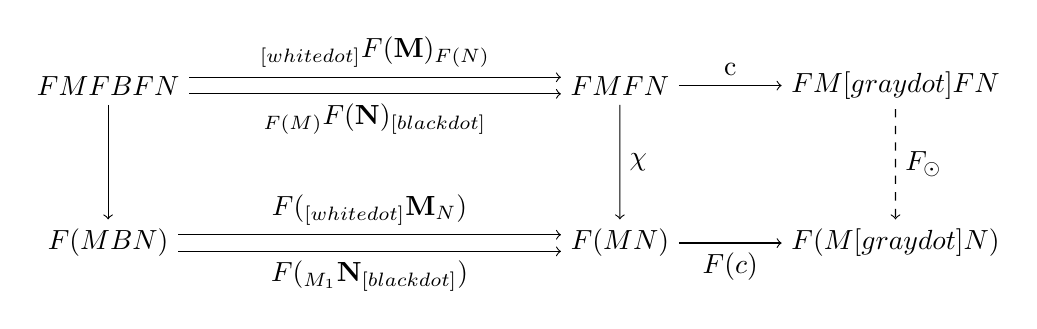
\begin{tikzpicture}[xscale=5, yscale=2, thin]
    \node (tl) at (-.3,1) {$FM \ten FB \ten FN$};
    \node (bl) at (-.3,0) {$F(M \ten B \ten N)$};
    \node (t) at (1,1) {$FM \ten FN$};
    \node (b) at (1,0) {$F(M\ten N)$};
    \node (tr) at (1.7,1) {$FM \tinydot[gray dot] FN$};
    \node (br) at (1.7,0) {$F(M \tinydot[gray dot] N)$};
    \draw[->] (tl) to node[left] {$\iso$} (bl);
    \draw[->] (t) to node[right] {$\chi \iso$} (b);
    \draw[->, dashed] (tr) to node[right] {$F_{\odot}$} (br);
    \draw[->] (t) to node[above] {c} (tr);
    \draw[->] (b) to node[below] {$F(c)$} (br);
    \draw[->] ([yshift=1.5pt]tl.east) to node[above] {${}_{\tinydot[white dot]}F(\mathbf{M})  \ten \mathid_{F(N)}$} ([yshift=1.5pt]t.west);
    \draw[->] ([yshift=-1.5pt]tl.east) to node[below] {$\mathid_{F(M)} \ten F(\mathbf{N})_{\tinydot[black dot]}$} ([yshift=-1.5pt]t.west);
    \draw[->] ([yshift=1.5pt]bl.east) to node[above] {$
    F({}_{\tinydot[white dot]}\mathbf{M} \tens \mathid_{N} )$} ([yshift=1.5pt]b.west);
    \draw[->] ([yshift=-1.5pt]bl.east) to node[below] {$F(\mathid_{M_1} \ten \mathbf{N}_{\tinydot[black dot]})$} ([yshift=-1.5pt]b.west);
  \end{tikzpicture}
 \end{equation}


The two commuting diagrams below show that $F_{\odot}$ is a module homomorphism and that $F_{\odot}$ is natural in $\mathbb{A}lg{\bf D}_1$.

\begin{equation}
\begin{tikzpicture}[xscale=2.5, yscale=2]
%uppersquare
\node (u1) at (1,3) [] {$F(A\otimes M \otimes N \otimes C)$};
\node (u2) at (3,3) [] {$F(A \otimes M \tinydot[gray dot] N \otimes C)$};
\node (u3) at (0,2.5) [] {$FA \ten FM \otimes FN \ten FC$};
\node (u4) at (2,2.5) [] {$FA \ten FM \tinydot[gray dot]FM \ten FC $};
\node (u-1) at (-1,3) [] {$F(A\otimes M \otimes B \ten N \otimes C)$};
\node (u-3) at (-2,2.5) [] {$FA \ten FM \otimes FB \ten FN \ten FC$};
%leftuppersquare
\draw[->] ([yshift=1.5pt]u-1.east) to node[above] {} ([yshift=1.5pt]u1.west);
    \draw[->] ([yshift=-1.5pt]u-1.east) to node[below] {} ([yshift=-1.5pt]u1.west);
        \draw[->] (u-3) to (u-1); 
 %%%   
\draw[->] (u1) to node[above] {} (u2);
\draw[->] (u3) to node[below] {} (u1); 
\draw[->, dashed ] (u4) to node[] {$\mathid \ten F_{\odot} \ten \mathid$} (u2);
%lowersquare
\node (m1) at (1,1.5) [] {$F(M \otimes N )$};
\node (m2) at (3,1.5) [] {$F(M \tinydot[gray dot] N) $};
\node (m3) at (0,1) [] {$FM \ten FN$};
\node (m4) at (2,1) [] {$FM \tinydot[gray dot] FN$};
\draw[->] (m3) to node[above] {} (m1); 
\draw[->, dashed] (m4) to node[] {$F_{\odot}$} (m2);
\draw[->] (m3) to node[above, xshift=8pt] {} (m4); 
\draw[->] (m1) to node[above] {} (m2);
\node (m-1) at (-1,1.5) [] {$F( M \ten B \ten N)$};
\node (m-3) at (-2,1) [] {$FM \ten  FB \ten FN $};
%leftlowersquare
\draw[->] ([yshift=1.5pt]m-1.east) to node[above] {} ([yshift=1.5pt]m1.west);
    \draw[->] ([yshift=-1.5pt]m-1.east) to node[below] {} ([yshift=-1.5pt]m1.west);
 \draw[->] ([yshift=1.5pt]m-3.east) to node[above] {} ([yshift=1.5pt]m3.west);
    \draw[->] ([yshift=-1.5pt]m-3.east) to node[below] {} ([yshift=-1.5pt]m3.west);
    \draw[->] (m-3) to (m-1);
%vertical
\draw[->] (u1) to node[] {$F({\bf M}_{\tinydot[gray dot]} \ten  {}_{\tinydot[gray dot]}{\bf N})$} (m1); 
\draw[->, dashed] (u2) to node[] {$F({\bf M}\tinydot[gray dot]{\bf N})$} (m2);
\draw[->, cross] (u3) to node[] {$F({\bf M})_{\tinydot[gray dot]} \ten {}_{\tinydot[gray dot]}F({\bf N})$} (m3); 
\draw[->, cross, dashed] (u4) to node[] {$F{\bf M }\tinydot[gray dot] F{\bf N}$} (m4);
\draw[->] (u-1) to node[] {$F({\bf M}_{\tinydot[gray dot]} \ten \mathid_B \ten {}_{\tinydot[gray dot]}{\bf N})$} (m-1);
\draw[->] (u-3) to node[above] {$F({\bf M})_{\tinydot[gray dot]} \ten \mathid_{FB} \ten {}_{\tinydot[gray dot]}F({\bf N})$} (m-3);
%%%% cross
\draw[->, cross] ([yshift=1.5pt]u-3.east) to node[above] {} ([yshift=1.5pt]u3.west);
    \draw[->, cross] ([yshift=-1.5pt]u-3.east) to node[below] {} ([yshift=-1.5pt]u3.west);
    \draw[->, cross] (u3) to node[above, xshift=8pt] {} (u4); 
\end{tikzpicture}
\end{equation}

\begin{equation}
\begin{tikzpicture}[xscale=2.5, yscale=2]
%uppersquare
\node (u1) at (1,3) [] {$F(M \otimes N)$};
\node (u2) at (3,3) [] {$F(M \tinydot[gray dot] N )$};
\node (u3) at (0,2.5) [] {$ FM \otimes FN $};
\node (u4) at (2,2.5) [] {$FM \tinydot[gray dot] FM$};
\node (u-1) at (-1,3) [] {$F(M \otimes B \ten N)$};
\node (u-3) at (-2,2.5) [] {$FM \otimes FB \ten FN$};
%leftuppersquare
\draw[->] ([yshift=1.5pt]u-1.east) to node[above] {} ([yshift=1.5pt]u1.west);
    \draw[->] ([yshift=-1.5pt]u-1.east) to node[below] {} ([yshift=-1.5pt]u1.west);
        \draw[->] (u-3) to (u-1); 
 %%%   
\draw[->] (u1) to node[above] {} (u2);
\draw[->] (u3) to node[below] {} (u1); 
\draw[->, dashed ] (u4) to node[] {$ F_{\odot}$} (u2);
%lowersquare
\node (m1) at (1,1.5) [] {$F(M' \otimes N' )$};
\node (m2) at (3,1.5) [] {$F(M' \tinydot[gray dot] N') $};
\node (m3) at (0,1) [] {$FM' \ten FN'$};
\node (m4) at (2,1) [] {$FM' \tinydot[gray dot] FN'$};
\draw[->] (m3) to node[above] {} (m1); 
\draw[->, dashed] (m4) to node[] {$F_{\odot}$} (m2);
\draw[->] (m3) to node[above, xshift=8pt] {} (m4); 
\draw[->] (m1) to node[above] {} (m2);
\node (m-1) at (-1,1.5) [] {$F(M' \ten B \ten N')$};
\node (m-3) at (-2,1) [] {$FM' \ten  FB \ten FN' $};
%leftlowersquare
\draw[->] ([yshift=1.5pt]m-1.east) to node[above] {} ([yshift=1.5pt]m1.west);
    \draw[->] ([yshift=-1.5pt]m-1.east) to node[below] {} ([yshift=-1.5pt]m1.west);
 \draw[->] ([yshift=1.5pt]m-3.east) to node[above] {} ([yshift=1.5pt]m3.west);
    \draw[->] ([yshift=-1.5pt]m-3.east) to node[below] {} ([yshift=-1.5pt]m3.west);
    \draw[->] (m-3) to (m-1);
%vertical
\draw[->] (u1) to node[] {$F(f \ten g)$} (m1); 
\draw[->, dashed] (u2) to node[] {$F(f \tinydot[gray dot] g)$} (m2);
\draw[->, cross] (u3) to node[] {$F(f) \ten F(g)$} (m3); 
\draw[->, cross, dashed] (u4) to node[] {$F(f) \tinydot[gray dot] F(g)$} (m4);
\draw[->] (u-1) to node[] {$F(f \ten \mathid \ten g)$} (m-1);
\draw[->] (u-3) to node[above] {$F(f) \ten \mathid \ten F(g)$} (m-3);
%%%% cross
\draw[->, cross] ([yshift=1.5pt]u-3.east) to node[above] {} ([yshift=1.5pt]u3.west);
    \draw[->, cross] ([yshift=-1.5pt]u-3.east) to node[below] {} ([yshift=-1.5pt]u3.west);
    \draw[->, cross] (u3) to node[above, xshift=8pt] {} (u4); 
\end{tikzpicture}
\end{equation}

One can show with a similar commuting diagram that $F_{\odot}$ is a natural isomorphism in $\mathbb{A}lg({\bf D})$.
The natural isomorphism $F_U: U_{F_0(A)} \rightarrow F_1(U_A)$. is a strict identity, by the definition of $U, \mathbb{A}lgF_0$, and $\mathbb{A}lgF_1$. Finally, it is straightforward that $S \circ F_1 = F_0 \circ S$ and $T \circ F_1 = F_0 \circ T$.

It remains to prove that the double functor $\mathbb{A}lgF$  is monoidal. The first condition i) is that $F_0$ and $F_1$ are strong monoidal functors, which comes down to showing that the natural transformations $\chi: \ten (F,F) \rightarrow  F\ten$ and $\iota: I_{\cD} \rightarrow F(I_{\cC})$ give rise to tight transformations of double categories, whose components are well-defined as algebra and module homomorphisms, respectively. This follows from naturality of $\chi$, and coherence and functoriality of $F$
Coherence of $\mathbb{A}lgF_0$ and $\mathbb{A}lgF_1$ follow from coherence of $F$. For condition ii) we need to show that $F_0 \circ S$ equals $S \circ F_1$ as monoidal functors, and similarly, $F_0 \circ T = T \circ F_1$. The first equality amounts to  $\chi^{F_0 \circ S} = \chi^{S \circ F_1}$ and $\chi^{F_0 \circ S} = \chi^{S \circ F_1}$, where we have written the functor that $\phi$ belongs to in superscript. Unfolding definitions gives us $F_0(\chi^{S}) \circ \chi^{F_0} = S(\chi^{F_1}) \circ \chi^{S}$. This holds, since $\chi^S$ is the identity. The other equalities are shown to hold in a similar way.

Finally, the first of the two additional diagrams given in condition (iii) of ~\ref{def:monfunc} corresponds to the front square of the commuting diagram below. The second can be shown to hold by a similar commuting diagram.

The unlabelled arrows represent the coequalisers defining their target object. The back square commutes by coherence of $F$. The squares on the sides commute by definition of $\xi$, $F_{\odot}$, and $\chi \tinydot[gray dot] \chi$ and by naturality of $\chi$. It follows that the fron square must commute.

\begin{equation}
\begin{tikzpicture}[xscale=3.2, yscale=2]
%lowersquare
\node (b1) at (0,0) [] {$F((N\ten L) \ten (M \ten K))$};
\node (b2) at (2,0) [] {$F((N \ten M) \ten (L \ten K))$};
\node (b3) at (1,-0.5) [] {$F((N\ten L) \tinydot[gray dot] (M \ten K))$};
\node (b4) at (3,-0.5) [] {$F((N \tinydot[gray dot] M) \ten (L \tinydot[gray dot] K))$}; 
\draw[->] (b1) to node[above, xshift=12pt] {$F(\hat{\sigma})$} (b2);
\draw[->] (b3) to node[above] {$F(\xi)$} (b4);
\draw[->] (b1) to node[above] {} (b3); 
\draw[->] (b2) to node[above] {} (b4);
%middlesquare
\node (m1) at (0,1.5) [] {$F(N\ten L) \ten F(M \ten K)$};
\node (m2) at (2,1.5) [] {$F(N \ten M) \ten F(L \ten K)$};
\node (m3) at (1,1) [] {$F(N\ten L) \tinydot[gray dot] F(M \ten K)$};
\node (m4) at (3,1) [] {$F(N \tinydot[gray dot] M) \ten F(L \tinydot[gray dot] K)$};
\draw[->] (m1) to node[above] {} (m3); 
\draw[->] (m2) to node[above] {} (m4);
%lowervertical
\draw[->] (m1) to node[left] {$\chi$} (b1); 
\draw[->] (m2) to node[left] {$\chi$} (b2);
\draw[->, cross] (m3) to node[left, yshift=8pt] {$F_{\odot}$} (b3); 
\draw[->] (m4) to node[left] {$\chi$} (b4);
%uppersquare
\node (u1) at (0,3) [] {$(FN \ten FL) \ten (FM \ten FK)$};
\node (u2) at (2,3) [] {$(FN \ten FM) \ten (FL \ten FK)$};
\node (u3) at (1,2.5) [] {$(FN \ten FL) \tinydot[gray dot] (FM \ten FK)$};
\node (u4) at (3,2.5) [] {$(FN \tinydot[gray dot] FM) \ten (FL \tinydot[gray dot] FK)$};
\draw[->] (u1) to node[left] {$\chi \ten \chi$} (m1); 
\draw[->] (u2) to node[left] {$\chi \ten \chi$} (m2);
\draw[->, cross] (u3) to node[left] {$\chi \tinydot[gray dot] \chi$} (m3); 
\draw[->] (u4) to node[left] {$F_{\odot} \ten F_{\odot}$} (m4);
\draw[->, cross] (u3) to node[above, xshift=8pt] {$\xi$} (u4); 
\draw[->] (u1) to node[above] {$\hat{\sigma}$} (u2);
\draw[->] (u1) to node[below] {} (u3); 
\draw[->, cross] (u2) to node[above] {} (u4);
\end{tikzpicture}
\end{equation}
\end{proof}  

\begin{thm}
Let $F:{\bf C} \rightarrow {\bf D}$ be a braided monoidal strong functor. The pseudofunctor of horizontal bicategories $\cAlg (F): \cAlg ({\bf C}) \rightarrow \cAlg ({\bf D})$ is braided monoidal strong. When $F$ is sylleptic, or symmetric, then $\cAlg (F)$ is sylleptic, or symmetric, respectively.
\end{thm}

\begin{proof}
Since $F$ is monoidal strong, the transformations $\chi$ and $\iota$ of $\mathbb{A}lg(F)$ are horizontally strong. The result follows from Proposition~\ref{prop:mfunctor} and Theorem~\ref{thm:lcbcfunctor}.
\end{proof}

Note that a similar result does not hold for braided monoidal lax or oplax functors, as the transformation $F_{\odot}$ will not be an isomorphism.

\begin{prop}\label{prop:mtrans}
Let $F,G: {\bf C} \rightarrow {\bf D}$ be braided monoidal functors. A monoidal transformation $\alpha: F \Rightarrow G$ lifts to a monoidal transformation $\bAlg \alpha: \bAlg F \Rightarrow \bAlg G$
\end{prop}

\begin{proof}
The components of any monoidal transformation $\alpha$ are algebra homomorphisms by the two coherence equations and by naturality of $\alpha$; hence, $\alpha$ gives rise to a natural transformation $\bAlg \alpha_0: \bAlg F_0 \Rightarrow \bAlg G_0$.
It gives rise to a natural transformation $\bAlg \alpha_1: \bAlg F_1 \Rightarrow \bAlg  G_1$, where the component $\alpha_{\bf M}$ of an $A-B-$Bimodule ${\bf M}$ is defined as $(\alpha_A, \alpha_M, \alpha_B)$. This is well-defined by naturality of $\alpha$ and the coherence equations for monoidal transformations.

The first equality for tight transformation follows from the first coherence condition for monoidal transformations, as shown below. Similarly, the second equality follows from the second coherence condition for monoidal tranformations.

\begin{equation}
\begin{tikzpicture}[xscale=2.5, yscale=2]
%uppersquare
\node (u1) at (1,3) [] {$F(M \otimes N)$};
\node (u2) at (3,3) [] {$F(M \tinydot[gray dot] N )$};
\node (u3) at (0,2.5) [] {$ FM \otimes FN $};
\node (u4) at (2,2.5) [] {$FM \tinydot[gray dot] FM$};
\node (u-1) at (-1,3) [] {$F(M \otimes B \ten N)$};
\node (u-3) at (-2,2.5) [] {$FM \otimes FB \ten FN$};
%leftuppersquare
\draw[->] ([yshift=1.5pt]u-1.east) to node[above] {} ([yshift=1.5pt]u1.west);
    \draw[->] ([yshift=-1.5pt]u-1.east) to node[below] {} ([yshift=-1.5pt]u1.west);
        \draw[->] (u-3) to (u-1); 
 %%%   
\draw[->] (u1) to node[above] {} (u2);
\draw[->] (u3) to node[below] {} (u1); 
\draw[->, dashed ] (u4) to node[] {$ F_{\odot}$} (u2);
%lowersquare
\node (m1) at (1,1.5) [] {$G(M \otimes N)$};
\node (m2) at (3,1.5) [] {$G(M \tinydot[gray dot] N) $};
\node (m3) at (0,1) [] {$GM \ten GN$};
\node (m4) at (2,1) [] {$GM \tinydot[gray dot] GN$};
\draw[->] (m3) to node[above] {} (m1); 
\draw[->, dashed] (m4) to node[] {$F_{\odot}$} (m2);
\draw[->] (m3) to node[above, xshift=8pt] {} (m4); 
\draw[->] (m1) to node[above] {} (m2);
\node (m-1) at (-1,1.5) [] {$G(M \ten B \ten N)$};
\node (m-3) at (-2,1) [] {$GM \ten  GB \ten GN $};
%leftlowersquare
\draw[->] ([yshift=1.5pt]m-1.east) to node[above] {} ([yshift=1.5pt]m1.west);
    \draw[->] ([yshift=-1.5pt]m-1.east) to node[below] {} ([yshift=-1.5pt]m1.west);
 \draw[->] ([yshift=1.5pt]m-3.east) to node[above] {} ([yshift=1.5pt]m3.west);
    \draw[->] ([yshift=-1.5pt]m-3.east) to node[below] {} ([yshift=-1.5pt]m3.west);
    \draw[->] (m-3) to (m-1);
%vertical
\draw[->] (u1) to node[] {$\alpha_{M \ten N}$} (m1); 
\draw[->, dashed] (u2) to node[] {$\alpha_{M \tinydot[gray dot] N}$} (m2);
\draw[->, cross] (u3) to node[] {$\alpha_M \ten \alpha_N$} (m3); 
\draw[->, cross, dashed] (u4) to node[] {$\alpha_M \tinydot[gray dot] \alpha_N$} (m4);
\draw[->] (u-1) to node[] {$\alpha_{M \ten B \ten N}$} (m-1);
\draw[->] (u-3) to node[above] {$\alpha_M \ten \alpha_B \ten \alpha_N$} (m-3);
%%%% cross
\draw[->, cross] ([yshift=1.5pt]u-3.east) to node[above] {} ([yshift=1.5pt]u3.west);
    \draw[->, cross] ([yshift=-1.5pt]u-3.east) to node[below] {} ([yshift=-1.5pt]u3.west);
    \draw[->, cross] (u3) to node[above, xshift=8pt] {} (u4); 
\end{tikzpicture}
\end{equation}

The coherence diagrams for monoidal transformations of double categories follow directly from the original coherence diagrams of $\alpha$.
\end{proof}

\begin{thm}
Let $\alpha: F \Rightarrow G$ be a braided monoidal natural isomorphism. The induced monoidal transformation of double categories $\bAlg \alpha: \bAlg F \Rightarrow \bAlg G$ lifts to a braided monoidal pseudo transformation $\cAlg \alpha: \cAlg F \Rightarrow \cAlg G$.
\end{thm}

\begin{proof}
As natural isomorphisms are loosely strong, the result follows from Proposition~\ref{prop:mtrans} and Theorem~\ref{thm:lcbcfunctor}.
\end{proof}

\subsection{$\cat 2()$}
We will extend the proof to the bicategory $2({\cat C})$ of dagger Frobenius algebras, dagger bimodules and bimodule homomorphisms in a braided monoidal category and demonstrate that it is braided monoidal and symmetric whenever ${\bf C}$ is symmetric.
\begin{defn}
A {\bf Frobenius algebra} is a monoidal category ${\cat C}$ is a monoid $(A, \tinymult, \tinyunit)$ together with a comonoid 
$(A, \tinycomult, \tinycounit)$ that satisfies the equations below.
\begin{align}
  \begin{pic}[]
    \node[gray dot] (t) at (.5,.5) {};
    \node[gray dot] (b) at (-.5,0) {};
    \draw (b.center) to[out=0,in=180] (t.center);
    \draw (-.5,-.5) to (b.center);
    \draw (t.center) to (.5,1);
    \draw (t.center) to[out=0,in=90] (1,-.5);
    \draw (-1,1) to[out=-90,in=180] (b.center);
  \end{pic}
\,=\,
  \begin{pic}[]
    \node[gray dot] (t) at (0,.5) {};
    \node[gray dot] (b) at (0,0) {};
    \draw (b.center) to (t.center);
    \draw (t.center) to[out=180,in=-90] (-.5,1);
    \draw (t.center) to[out=0,in=-90] (.5,1);
    \draw (b.center) to[out=180,in=90] (-.5,-.5);
    \draw (b.center) to[out=0,in=90] (.5,-.5);
  \end{pic}
 \, =\,
  \begin{pic}[]
    \node[gray dot] (t) at (-.5,.5) {};
    \node[gray dot] (b) at (.5,0) {};
    \draw (b.center) to[out=180,in=0] (t.center);
    \draw (.5,-.5) to (b.center);
    \draw (t.center) to (-.5,1);
    \draw (t.center) to[out=180,in=90] (-1,-.5);
    \draw (1,1) to[out=-90,in=0] (b.center);
  \end{pic}
\end{align}
We call a Frobenius algebra {\bf special} whenever the following equation holds.
 \begin{align}
  \begin{pic}[]
        \node (0) at (0,-0.5) {};
        \node[gray dot] (1) at (0,-.1) {};
        \node[gray dot] (2) at (0,0.6) {};
        \node (3) at (0,1) {};
        \draw (0.center) to (1.center);
        \draw (2.center) to (3.center);
        \draw[in=180, out=180, looseness=2] (1.center) to (2.center);
        \draw[in=0, out=0, looseness=2] (1.center) to (2.center);
\end{pic}
\,=\,
  \begin{pic}[]
    \draw (0,-.5) to (0,1);
  \end{pic}
\end{align}
\end{defn}



\begin{rmk}\label{comspecfrob}
The bicategory of Frobenius algebras, bimodules and bimodule homomorphisms is symmetric monoidal. This follows from Theorem ~\ref{thm:eqcomp} since Frobenius algebras and algebra homomorphisms form a full symmetric monoidal subcategory of the category of algebras and algebra homomorphisms. The same statement holds for special and commutative Frobenius algebras. 
\end{rmk}


\begin{defn}
Let {\bf C} be a braided monoidal category. A dagger functor $\dagger: {\cat C} \rightarrow {\cat C}$, a contravariant functor which is the identity on objects. A Frobenius algebra in {\cat C} is a {\bf dagger Frobenius algebra} when the coalgebra is the dagger image of the algebra. 
A bimodule is called a {\bf dagger bimodule} when the equation below holds, where we denote $\dagger({\bf M})$ by ${\bf M}^{\dagger}$.

\begin{align}
    \begin{pic}[yscale=.85]
      \node[morphism, minimum width=10mm] (m) at (0,-.7) {$\textbf{M}^\dag$};
      \draw (m.south) to (0,-2) node[right]{$M$};
      \draw (m.north) to  (0,.6) node[right]{$M$};
      \draw (m.45) to[out=90,in=-90] (.5,.6) node[right]{$D$};
      \draw (m.135) to[out=90,in=-90] (-.5,.6) node[right]{$C$};
    \end{pic}
    \!\!\!=\,\,\,
    \begin{pic}[yscale=.85]
      \node[morphism, minimum width=10mm] (m) at (0,-.7) {$\textbf{M}$};
      \draw (m.south) to (0,-2) node[right]{$M$};
      \draw (m.north) to (0,.6) node[right]{$M$};
      \node[white dot] (l) at (-.6,-1.3) {};
      \node[black dot] (r) at (.6,-1.3) {};
      \draw (m.-45) to[out=-90,in=150] (r);
      \draw (m.-135) to[out=-90,in=30] (l);
      \draw (r) to (.6,-1.6) node[black dot] {};
      \draw (l) to (-.6,-1.6) node[white dot] {};
      \draw (l) to[out=150, in=-90, looseness=.5] (-1,.6) node[right] {$C$};
      \draw (r) to[out=30, in=-90, looseness=.5] (1,.6) node[right] {$D$};
    \end{pic}
    \end{align}
\end{defn}
When a braided monoidal category {\bf C} is equiped with a dagger functor, dagger Frobenius algebras and dagger bimodules and bimodule homomorphisms do not form a fibrant double category by the method introduced in this paper. The reason is that the bimodule defined in equation ~\ref{eq:companion} as part of the data that forms a companion is not a dagger bimodule. To solve this, we restrict the categories $\mathbb{D}_0$ and $\mathbb{D}_1$ in an appropriate way to ensure that the result still holds.

\begin{defn}
Let $f: A\rightarrow B$ be an algebra homomorphism in a dagger category. The {\bf conjugate} $f_*$ of $f$ is defined as 
\begin{align*}
f_* :=
\begin{pic}[]
    \node[gray dot] (t) at (.5,.8) {};
    \node[gray dot] (b) at (-.5,-.3) {};
    \node[gray dot] (tu) at (.5,1){};
    \node[gray dot] (bu) at (-.5,-.5){};
    \node[morphism, minimum width=10mm] (m) at (0,.25) {$f^{\dagger}$};
    \draw (b.center) to[out=0, in=-90] (m.south);
    \draw (m.north) to[out=90, in=180] (t.center);
    \draw (-.5,-.5) to (b.center);
    \draw (t.center) to (.5,1);
    \draw (t.center) to[out=0,in=90] (1,-.5);
    \draw (-1,1) to[out=-90,in=180] (b.center);
  \end{pic}
\end{align*}

An algebra homomorphism $f$ is {\bf self-conjugate} if $f=f_*$.
\end{defn}

\begin{prop}\label{prop:dagger}
Let ${\cat C}$ be a braided monoidal dagger category. The bicategory $2({\cat C})$ of dagger Frobenius algebras, dagger bimodules and bimodule homomorphisms of ${\cat C}$ is braided monoidal; it is symmetric whenever {\bf C} is symmetric.
\end{prop}

\begin{proof}
The bicategory is the horizontal bicategory of the double category of dagger Frobenius algebras and self-conjugate algebra homomorphisms, dagger bimodules and extended bimodule homomorphisms $(f_1,f,f_2)$ in {\cat C}, of which $f_1$ and $f_2$ are self-conjugate. This ensures that ~\ref{eq:companion} is a dagger bimodule.  This is a symmetric monoidal subcategory of our original double category, since self-conjugate morphisms are closed under the tensor product and all structure isomorphisms of the monoidal double category are self-conjugate. Applying Theorem~\ref{thm:H} on this double category give the required result.
\end{proof}

\begin{cor}
The bicategory $2Hilb$ defined in ~\cite{baez} is symmetric monoidal.
\end{cor}

\begin{proof}
$2Hilb$ is a full subcategory of 2(Hilb). [details needed]
\end{proof}


\begin{cor}
Let ${\bf C}$ be a symmetric monoidal category. The bicategory $2(CP({\bf C}))$ of ~\cite{heunenvicarywester} is symmetric monoidal.
\end{cor}

\begin{proof}
This follows directly from proposition \ref{prop:dagger}.
\end{proof}

\begin{prop}
Let ${\bf C, D}$ be braided monoidal dagger categories, let $F:{\bf C} \rightarrow {\bf D}$ be a braided monoidal strong dagger functor that preserves coequalisers. The functor $F$ lifts to a braided monoidal strong pseudofunctor $2(F): 2({\bf C}) \rightarrow 2({\bf D})$.
\end{prop}
  
\begin{proof}
The braided monoidal dagger functor $F$ preserves special dagger Frobenius algebras, self-conjugate algebra homomorphisms and dagger bimodules. As a result, the braided monoidal functor $\mathbb{A}lgF: \mathbb{A}lg{\bf C} \rightarrow \mathbb{A}lg{\bf D}$ restricts to a braided monoidal functor between the full monoidal subcategories $\mathbbm{2}(F): \mathbbm{2}({\bf C}) \rightarrow \mathbbm{2}({\bf D})$. As the structure transformations $\chi, \iota$ are horizontally strong, $\mathbbm{2}(F)$ lifts to a braided monoidal strong pseudofunctor $2(F): 2({\bf C}) \rightarrow 2({\bf D})$ by Theorem~\ref{thm:H}.
\end{proof}

\begin{thm}
Let $F,G: {\bf C} \rightarrow {\bf D}$ be braided monoidal strong functors that preserve coequalisers. Any braided monoidal natural isomorphism $\alpha: F \Rightarrow G$ lifts to a braided monoidal pseudo natural adjoint equivalence $2(\alpha):  2(F) \Rightarrow 2(G)$.  
\end{thm}

\begin{proof}
We obtain the result by restricting the braided monoidal isomorphism of double functors $\bAlg \alpha$ to its components in $\mathbbm{2}({\bf C})$ to obtain a braided monoidal double isomorphism $\mathbbm{2}(\alpha): \mathbbm{2}(F) \rightarrow \mathbbm{2}(G)$. This isomorphism lifts to a braided monoidal pseudo adjoint equivalence $2(\alpha); 2(F) \rightarrow 2(G)$ by Theorem~\ref{thm:h-locfr}.
\end{proof}
% Local Variables:
% TeX-master: "smbicat"
% End:
